\chapter{A Riemannian Manifold Optimization Framework for CMA}
\label{chap:RTR}

Riemannian Manifold Optimization, first introduced by Absil \cite{Absil2008book}, has gained a lot of attention due to its capability to handle problems with a real-valued objective function defined on a constrained space,
\begin{equation}
\underset{\bm{M}\in\mathbb{C}^{m\times n}}{\text{minimize}}\quad f({\bm{M}})\quad\text{s.t.}\quad\bm{M}\in\mathcal{M},
\end{equation} where the space $\mathcal{M}$ might not be well-defined in terms of addition, continuity, and/or other properties exploited by regular optimization approaches in Euclidean spaces. The main idea is to redefine the problem as an unconstrained optimization problem over a space known as a manifold. Manifolds are topological spaces that -equipped with a metric- locally resemble Euclidean spaces of the same dimensionality, but might be remarkably different in global terms.
%Manifolds are topological spaces that locally resemble Euclidean space of the same dimensionality near each point. In particular, a smooth manifold is defined as a set $\bm{M}$ that locally resembles Euclidean space of the same dimensionality, but can be very different in global terms, where the smoothness plays a key role in the application of classical optimization procedures. 
Some manifold examples include spheres, the set of rotations, the set of positive semidefinite matrices, the set of fixed-rank matrices, among many others. The application of Riemannian manifold optimization techniques has shown success in several fields, such as low-rank matrix decomposition \cite{Yang2016lowrankfogran}, phase retrieval \cite{}, blind signal demixing \cite{Dong2018b}, dictionary learning \cite{}, among others.

%Succinctly, a manifold optimization approach generalizes the Euclidean gradient (Hessian) to a Riemannian gradient (Hessian), such that
%\begin{align}
%\underbrace{\text{grad}_{\bm{M}_t}f(\bm{M}_t)}_{\text{Riemannian gradient}}&=P_{\bm{M}_t}\big(\underbrace{\nabla f(\bm{M}_t)}_{\text{Euclidean gradient}}\big)\\
%\nonumber\\
%\underbrace{\text{Hess}_{\bm{M}_t}f(\bm{M}_t)[\bm{\eta}_{\bm{M}_t}]}_{\text{Riemannian Hessian}}&=P_{\bm{M}_t}\big(\nabla^2f(\bm{M}_t)[\bm{\eta}_{\bm{M}_t}]\big)\\
%\nonumber\\
%\bm{M}_{t+1}&=\mathcal{R}_{\bm{M}_{t}}\big(-\alpha_k\cdot\text{grad}_{\bm{M}_t}f(\bm{M}_t)\big)
%\end{align}
%where $P_{\bm{M}}(\cdot)$ is the projection operator into the tangent space $T_{\bm{M}}\mathcal{M}$, $\nabla^2f(\bm{M}_t)[\bm{\eta}_{\bm{M}_t}]$ is the directional derivative of the Euclidean gradient in direction $\bm{\eta}_{\bm{M}_t}$, and $\mathcal{R}_{\bm{M}}(\cdot)$ is the retraction operator that takes the update rule back to the manifold.
%
%With this in mind, we can transform $\mathcal{P}$ into a manifold optimization problem following the procedure in \cite{Dong2018b}.

\section{Redefining the CMA Problem}
%Knowing that $\bm{w}\herm\bm{X}_{k}\bm{w}=\mathrm{Tr}(\bm{w}\herm\bm{X}_{k}\bm{w})=\mathrm{Tr}(\bm{X}_{k}\bm{ww}\herm)=\text{Tr}(\bm{X}_{k}\bm{W})=\mathrm{Tr}(\bm{X}_{k}\herm\bm{W})=\langle\bm{X}_{k},\bm{W}\rangle$, with $\langle\cdot,\cdot\rangle$ the matrix inner product, we can rewrite $\mathcal{P}$ as 
%\begin{eqnarray}
%\mathcal{P}:\,\,\underset{\bm{W}\in\mathbb{S}_+^{M}}{\text{minimize}}\quad& g(\bm{W})=\displaystyle{\frac{1}{K}\sum_{k=1}^K\Big(\mathrm{Tr}(\bm{X}_{k}\bm{W})-1\Big)^2}\nonumber\\
%\text{s.t.}\quad&\text{rank}(\bm{W})=1,
%\end{eqnarray}
%where $\mathbb{S}_+^{M}$ is the set of Hermitian positive semidefinite matrices of size $M\times M$. 
%We can then define a linear map $h:\mathbb{S}_+^{M}\rightarrow\mathbb{R}^K$ such that
%\begin{equation}
%\big[h(\bm{W})\big]_k=\mathrm{Tr}(\bm{X}_{k}\bm{W})=\langle\bm{X}_{k},\bm{W}\rangle,
%\end{equation}
%and $\bm{1}$ as the vector whose elements are all equal to 1. Now let $\mathcal{M}$ be the non-compact manifold encoded with the rank-one matrices, so exploiting the Riemannian manifold geometry $\mathcal{P}$ can be transformed into the following unconstrained optimization problem over the search space of $\mathcal{M}$:
%\begin{eqnarray}
%\mathcal{P}':\,\,\underset{\bm{W}\in\mathcal{M}}{\text{minimize}}\quad g(\bm{W})=\displaystyle{\frac{1}{K}\Big\|h(\bm{W})-\bm{1}\Big\|^2}
%\end{eqnarray}
%We can further reduce the dimensionality of the search space by using the known factorization for rank-one Hermitian positive semidefinite matrices $\bm{W}=\bm{ww}\herm,\,\bm{w}\in\mathbb{C}_*^M$ \cite{}. Hence, we can rewrite $\mathcal{P}$ as
%The CMA problem \ref{eqn:cma} can be subtly rewritten as
%\begin{eqnarray}
%\mathcal{P}:\,\,\underset{\bm{w}\in\mathcal{C}}{\text{minimize}}\quad f(\bm{w})=\displaystyle{\frac{1}{K}\sum_{k=1}^K\Big(\bm{w}\herm\bm{X}_{k}\bm{w}-1\Big)^2}
%\end{eqnarray}
%where $\mathcal{C}=\mathbb{C}_*^M$ is the set of complex vectors of size $M$ without the zero-vector.
%Even if this seems redundant, it's important to note that the computational space is not longer Euclidean globally, but can be described as a manifold.

The CMA problem (\ref{eqn:cma}), as an unconstrained problem, implies that there is no restriction on the search space $\mathbb{C}^M$, and we can consider this space as a Riemannian manifold when endowed with an inner product, also known as Riemannian metric, which will be discussed later. However, the CMA problem is phase-invariant, which means that all rotations of its solution are also solutions, i.e. $|\bm{w}\herm\bm{x}_{k}|^2=|(\alpha\bm{w})\herm\bm{x}_{k}|^2$ with $\alpha\in\text{U}(1)=\{\alpha\in\mathbb{C}:|\alpha|=1\}$, where $\text{U}(1)$ is the unitary group of degree 1, and thus solutions are not unique. Second-order optimization techniques usually require non-degenerate critical points to perform as expected, which in turn is related to the uniqueness of such critical points \cite{}. Hence, we define the relation $\bm{w}\mapsto[\bm{w}]$, which forms an equivalence class
\begin{equation}
[\bm{w}]=\{\alpha\bm{w}:\alpha \in \text{U}(1)\}.\label{eqn:equivalenceclass}
\end{equation}

When this equivalence class is considered in the manifold $\mathcal{C}$, we obtain an abstract space known as a quotient manifold $\mathcal{C}/{\sim}=\mathbb{C}^M/\text{U}(1)$, where the rotation of vectors are all assigned to one vector, thus avoiding the scalar indetermination of the problem. 

\subsection{Riemannian Geometry}

The quotient manifold $\mathcal{C}/{\sim}$ is an abstract space, and thus requires matrix representations in the computational space $\mathcal{C}$. An element ${\bm{w}}_q$ in the quotient manifold can be represented by an element $\bm{w}$ in the computational space, thus every geometry-related operation over the quotient manifold can be defined in terms of elements and operations in the computational space.
In particular, we need to define length with a Riemannian metric $d_{\bm{w}}$, a set of directional derivatives called the horizontal space $\mathcal{H}_{\bm{w}}$, the motion along the manifold known as retraction $\mathcal{R}_{\bm{w}}$, and other optimization-related formulas such as gradients and Hessians. 

The first step is to derive a Riemannian metric, which is defined at each element $\bm{w}$ for elements of the tangent space $\mathcal{T}_{\bm{w}}\mathcal{C}$, shall be a smooth inner product $d_{\bm{w}}(\bm{u}_{\bm{w}},\bm{v}_{\bm{w}})$ suited for the computational space $\mathcal{C}$ (where $\bm{u}_{\bm{w}},\bm{v}_{\bm{w}}\in\mathcal{T}_{\bm{w}}\mathcal{C}$). In our case, that inner product is the real-trace metric given by
\begin{equation}
d_{\bm{w}}(\bm{u}_{\bm{w}},\bm{v}_{\bm{w}})=2\Re\Big(\Tr(\bm{u}_{\bm{w}}\herm\bm{v}_{\bm{w}})\Big)=\Tr\big(\bm{u}_{\bm{w}}\herm\bm{v}_{\bm{w}}+\bm{v}_{\bm{w}}\herm\bm{u}_{\bm{w}}\big).
\end{equation} 

The tangent space can be characterized as the direct sum of two orthogonal spaces known as \emph{horizontal space} $\mathcal{H}_{\bm{w}}\mathcal{C}$ and \emph{vertical space} $\mathcal{V}_{\bm{w}}\mathcal{C}$. The latter contains the vectors representing directions tangent to the the set of the equivalence class (\ref{eqn:equivalenceclass}). Then, the horizontal space consists of the directions orthogonal to the equivalence class, and therefore the elements of the tangent space can be represented by an unique element belonging to the horizontal space. This forms a Riemannian submersion from the quotient manifold to the computational space, thus defining a correspondence between elements of the quotient space and elements of the computational space \cite{Absil2008book}.
Under these considerations, the geometric definitions for the Riemannian optimization of CMA are shown in Table~\ref{table:riemmann}.

\subsection{Riemannian Optimization for CMA}

We use a Riemannian Trust-Region (RTR) algorithm, which is a second-order optimization approach with superlinear convergence rate \cite{Absil2007trustregions}. The algorithm searches the direction $\bm{\eta}_{\bm{w}}$ on the horizontal space $\mathcal{H}_{\bm{w}}\mathcal{C}$. At each iteration we solve the trust-region subproblem with $\bm{w}\in\mathcal{C}$ 
\begin{eqnarray}
\mathcal{Q}:\,\,\underset{\bm{\eta}_{\bm{w}}\in\mathcal{H}_{\bm{w}}\mathcal{C}}{\text{minimize}}\quad& q(\bm{\eta}_{\bm{w}})=d_{\bm{w}}\big(\bm{\eta}_{\bm{w}},\text{grad}_{\bm{w}}f(\bm{w})\big)+\frac{1}{2}d_{\bm{w}}\big(\bm{\eta}_{\bm{w}},\text{Hess}_{\bm{w}}f(\bm{w})[\bm{\eta}_{\bm{w}}]\big)\nonumber\\
\text{s.t.}\quad&d_{\bm{w}}(\bm{\eta}_{\bm{w}},\bm{\eta}_{\bm{w}})\leq\delta^2
\end{eqnarray}
where $\bm{\eta}_{\bm{w}}$ is in the horizontal space of iterate $\bm{w}$, $\delta$ denotes the trust region radius, 
%and the cost function is given by
%\begin{equation}
%q(\bm{\eta}_{\bm{w}})=d_{\bm{w}}\big(\bm{\eta}_{\bm{w}},\text{grad}_{\bm{w}}f(\bm{w})\big)+\frac{1}{2}d_{\bm{w}}\big(\bm{\eta}_{\bm{w}},\text{Hess}_{\bm{w}}f(\bm{w})[\bm{\eta}_{\bm{w}}]\big)
%\end{equation}
%with 
$\text{grad}_{\bm{w}}f(\bm{w})$ the Riemannian gradient and $\text{Hess}_{\bm{w}}f(\bm{w})[\bm{\eta}_{\bm{w}}]$ the Riemannian Hessian, respectively. 
For the CMA-based single source recovery scenario, the Riemannian gradient of $f$ is given by
\begin{align}
\mathrm{grad}_{\bm{w}}f(\bm{w})=\frac{2}{K}\sum_{k=1}^K \big(|\bm{w}\herm\bm{x}_k|^2-1\big)\bm{x}_k\bm{x}_k\herm\bm{w}, \label{eqn:rtrgradient}
\end{align}
and the Riemannian Hessian in direction $\bm{\eta}_{\bm{w}}$ is
\begin{align}
\Hess f(\bm{w})[\bm{u}]=\frac{2}{K}\sum_{k=1}^K\bigg( \big(\bm{w}\herm\bm{X}_k\bm{u}_{\bm{w}}+\bm{u}_{\bm{w}}\herm\bm{X}_k\bm{w}\big)\bm{X}_k\bm{w} +\big(|\bm{w}\herm\bm{x}_k|^2-1\big)\bm{X}_k\bm{u}\bigg).\label{eqn:rtrhessian}
\end{align}
where $\bm{X}_k=\bm{x}_k\bm{x}_k\herm$. These expressions are derived in Appendix~\ref{appdxrtr:riemannDerivations}.

\begin{table*}
	\normalsize\centering
	\caption{Riemannian geometry definitions required for manifold optimization of the CMA Problem.} \label{table:riemmann}
	\begin{tabular}{l|l}
		Name&Definition\\\hline
		Computational space $\mathcal{C}$   & $\mathbb{C}^M$\\
		Quotient space $\mathcal{C}/{\sim}$   & $\mathbb{C}^M/\mathrm{U}(1)$\\
		Riemannian metric $d_{\bm{w}}$ & $d_{\bm{w}}(\bm{u}_{\bm{w}},\bm{v}_{\bm{w}})=\mathrm{Tr}(\bm{u}_{\bm{w}}\herm\bm{v}_{\bm{w}}+\bm{v}_{\bm{w}}\herm\bm{u}_{\bm{w}})$\\
		Horizontal space $\mathcal{H}_{\bm{w}}\mathcal{C}$ & $\mathcal{H}_{\bm{w}}\mathcal{C}=\{\bm{\eta}_{\bm{w}}\in\mathbb{C}^M:\bm{\eta}_{\bm{w}}\herm\bm{w}=\bm{w}\herm\bm{\eta}_{\bm{w}}\}$\\
		Horizontal space projection $\Pi_{\mathcal{H}_{\bm{w}}\mathcal{C}}$& $\Pi_{\mathcal{H}_{\bm{w}}\mathcal{C}}(\bm{\eta}_{\bm{w}})=\bm{\eta}_{\bm{w}}-a\bm{w},\,\,a=(\bm{w}\herm\bm{\eta}_{\bm{w}}-\bm{\eta}_{\bm{w}}\herm\bm{w})/2\bm{w}\herm\bm{w}$ \\
		Riemannian gradient $\mathrm{grad}_{\bm{w}}f$ & $\mathrm{grad}_{\bm{w}}f(\bm{u}_{\bm{w}})=\Pi_{\mathcal{H}_{\bm{w}}\mathcal{C}}\big(\frac{1}{2}\nabla_{\bm{w}}f(\bm{u}_{\bm{w}})\big)$\\
		Riemannian Hessian $\mathrm{Hess}_{\bm{w}}f$ & $\mathrm{Hess}_{\bm{w}}f(\bm{w})[\bm{\eta}_{\bm{w}}]=\Pi_{\mathcal{H}_{\bm{w}}\mathcal{C}}\big(\frac{1}{2}\nabla^2_{\bm{w}}f(\bm{u}_{\bm{w}})[\bm{\eta}_{\bm{w}}]\big)$\\
		Retraction $\mathcal{R}_{\bm{w}}$ & $\mathcal{R}_{\bm{w}}(\bm{u}_{\bm{w}})=\bm{w}+\bm{u}_{\bm{w}}$\\
	\end{tabular}
\end{table*}

With the above derivations and the formulas from Table~\ref{table:riemmann}, we can define the RTR algorithm as summarized in Algorithm~\ref{alg:rtr}. Succinctly, in each iteration we solve the trust-regions subproblem $\mathcal{Q}$ in the horizontal space of the current iterate, obtaining a descent direction $\bm{\eta}_{\bm{w}}$ in the horizontal space, whose magnitude is given by the size of the accepted trust region \cite{Absil2008book}. The next iterate is computed using the retraction of $\bm{\eta}_{\bm{w}}$, which brings the result back to the manifold.
\begin{algorithm}[H]
	\caption{Riemannian Trust-Region for CMA-based Single Source Beamforming}
	\label{alg:rtr}
	\begin{algorithmic}[1]
		\Statex {\textbf{Given: }Received signals $\bm{x}_{k}\in\mathbb{C}^M,\,k=1,\ldots,K$, Riemannian manifold $\mathcal{C}$ with metric $d_{\bm{w}}$, Riemannian gradient $\grad$, Riemannian Hessian $\Hess$, retraction $\mathcal{R}_{\bm{w}}$, and objective function $f$}
		\Statex \textbf{A) Initialization:} 
		\State Define $t=0$ and $\displaystyle \bm{w}_0$
		\Statex \textbf{B) Trust Region:}
		\While{not converged}
		\State Obtain descent direction $\bm{\eta}_{\bm{w}_t}$ by solving $\mathcal{Q}$ in $\mathcal{H}_{\bm{w}_t}\mathcal{C}$
		\State $\displaystyle \bm{w}_{t+1}=\mathcal{R}_{\bm{w}_t}\big(\bm{\eta}_{\bm{w}_t}\big)$
		\EndWhile
	\end{algorithmic}
\end{algorithm}

A known algorithm to solve the trust-region subproblem $\mathcal{Q}$ based in a truncated Conjugate Gradient approach is presented in Algorithm~11 in \cite[Section 7.3]{Absil2008book}. A variation of this algorithm has been implemented in the manifold optimization toolbox Manopt \cite{manopt}. We use this open-source toolbox to implement Algorithm~\ref{alg:rtr}, exploiting its flexibility for selectable choices for stopping criteria, tolerances, and other parameters.

\subsection{Riemannian Geometry for CMA-based Multiple Signal Recovery}

For the multiple signal recovery scenario, a few modifications are needed. First, as each combiner can be treated independently from each other, we can define a new topology known as a product manifold, which is the aggregation of the manifolds containing each variable as a Cartesian product. The matrix representation of the product manifold is obtained as the Cartesian product of the sets that represent each manifold. Formally, we define the product manifold $\mathcal{C}^J=\mathcal{C}\times\ldots\times\mathcal{C}, \, J$ times, as the set of tuples $(\bm{w}_1,\ldots,\bm{w}_J)$ with $\bm{w}_j\in\mathcal{C},\,j=\{1,\ldots,J\}$.
We can also define an equivalence class to avoid the scalar indetermination in each manifold as:
\begin{equation}
[\bm{b}]=\{[\bm{w}_j]\}_{j=1}^J,\,\,\text{with }[\bm{w}_j]=\{\alpha_j\bm{w}_j:\alpha_j \in \text{SU}(1)\},\label{eqn:equivalenceclass_msr}
\end{equation}
obtaining a new quotient product manifold $\mathcal{C}^J/{\sim}$ (where we abuse the notation of the equivalence class for notational simplicity). Thus, the geometry definitions of Table~\ref{table:riemmann} are sufficient to describe the geometry of the quotient product manifold. Therefore, the same Riemannian optimization procedures and algorithms can be used for this extended problem, and we only need to find the Riemannian gradient and Hessian for this case. The Riemannian gradient with respect to the $j$-th combiner is given by
\begin{align}
\mathrm{grad}_{\bm{w}_j}g(\bm{b})=\frac{2}{K}\sum_{k=1}^K (\bm{w}_j\herm\bm{X}_k\bm{w}_j-1)\bm{X}_k\bm{w}_j + \gamma_0\sum_{j_1\neq j}\bm{O}\bm{w}_{j_1}\bm{w}_{2}\herm\bm{O}\bm{w}_j, \label{eqn:rtrgradient_msr}
\end{align}
and the corresponding Riemannian Hessian in direction $\bm{\eta}_{\bm{w}_j}$ is
\begin{align}
\Hess_{\bm{w}_j} g(\bm{b})[\bm{\eta}_{\bm{w}_j}]
&=\frac{2}{K}\sum_{k=1}^K \big(\bm{\eta}_{\bm{w}_j}\herm\bm{X}_k\bm{w}_j+\bm{w}_j\herm\bm{X}_k\bm{u}_{\bm{w}})\bm{X}_k\bm{w}_j+\frac{2}{K}\sum_{k=1}^K \big(\bm{w}_j\herm\bm{X}_k\bm{w}_j-1\big)\bm{X}_k\bm{\eta}_{\bm{w}_j}\nonumber\\
&\quad+\gamma_0\sum_{j_1\neq j}^J\bigg(\bm{O}\bm{w}_{j_1}\bm{w}_{j_1}\herm\bm{O} \bm{\eta}_{\bm{w}_j}+\bm{O}\big(\bm{\eta}_{\bm{w}_j}\bm{w}_{j_1}\herm +\bm{w}_{j_1}\bm{\eta}_{\bm{w}_{j_1}}\herm\big)\bm{O}\bm{w}_j\bigg)\label{eqn:rtrhessian_msr}
\end{align}
where $\bm{O}$ is the sample covariance of the received signals $\bm{x}_k$, i.e. $\bm{O}=K^{-1}\sum_k\bm{x}_k\bm{x}_k\herm$.
These expressions are also derived in Appendix~\ref{appdxrtr:riemannDerivations}.

With the above derivations and the formulas from Table~\ref{table:riemmann}, we can define the RTR algorithm as summarized in Algorithm~\ref{alg:rtr_msr}. This algorithm follows the same structure of the single source recovery case, but includes several calls to the trust-regions subproblem to compute the iterate of each manifold that composes the product manifold.
\begin{algorithm}[H]
	\caption{Riemannian Trust-Region for CMA-based Multiple Source Beamforming}
	\label{alg:rtr_msr}
	\begin{algorithmic}[1]
		\Statex {\textbf{Given: }Received signals $\bm{x}_{k}\in\mathbb{C}^M,\,k=1,\ldots,K$, Riemannian manifold $\mathcal{C}$ with metric $d_{\bm{w}}$, Riemannian gradients $\grad$, Riemannian Hessians $\Hess$, retractions $\mathcal{R}_{\bm{w}}$, and objective function $g$}
		\Statex \textbf{A) Initialization:} 
		\State Define $t=0$ and $\displaystyle \bm{w}_j^0$, $j\in\{1,\ldots,J\}$
		\Statex \textbf{B) Trust Region:}
		\While{not converged}
		\For{$j\in\{1,\ldots,J\}$}
		\State Obtain descent directions $\bm{\eta}_{\bm{w}_j^t}$ by solving $\mathcal{Q}$ in $\mathcal{H}_{\bm{w}_j^t}\mathcal{C}$
		\State $\displaystyle \bm{w}_{j}^{t+1}=\mathcal{R}_{\bm{w}_j^t}\big(\bm{\eta}_{\bm{w}_j^t}\big)$
		\EndFor
		\EndWhile
	\end{algorithmic}
\end{algorithm}

Now, note that our computational spaces are Euclidean spaces, so this is essentially no different from trust-regions algorithms for CMA problems \cite{Kreutz2008trustregionscma}, and additionally, the Riemannian manifold approach could be overly complicated for our case (as the original manifold is a Euclidean space). Nevertheless, understanding this approach allows us to explore different manifolds that might be well suited for the CMA problem. One example for Multiple User Recovery is to use noncompact Stiefel manifolds (i.e., matrices with linearly independent columns) to force the statistical independence of the different combiners when grouped as the columns of one matrix, instead of regularizing the cost function with the sample covariance of the equalized signals. These potential applications are a motivation to properly derive Riemannian manifold optimization techniques and different geometries for blind equalization.



\section{Convergence Analysis} \label{convergence_rtr}
Trust-region optimization methods are a class of optimization algorithms that have both global convergence properties and local convergence with superlinear rate. Additionally, they are known to reduce the computational complexity of plain Newton methods when the iterates are far from the solution, and are thus desirable for matrix manifold optimization. %A trust-region method has been studied for phase retrieval in \cite{Sun2016geometricgpr}.
The Riemannian Trust-Region algorithm presented as-is in~\cite{Absil2007trustregions} has provable global and local convergence properties, as long as some conditions on the cost function and manifold geometry are met. Here, we show that the CMA problem satisfy both global and local convergence for RTR.

\subsection{Global convergence}
This property ensures that the sequence of iterates $\{\bm{w}_t\}$ generated by RTR converges to the set of stationary points of the cost function, i.e., $
\lim_{t\rightarrow\infty}\|\grad f(\bm{w}_t)\|=0$.
In particular, \cite[Corollary 4.6]{Absil2007trustregions} states that if the cost function and retraction operator are smooth, and the Riemannian manifold is compact, then all the conditions for global convergence properties of RTR are satisfied. Note that, technically, this corollary only needs to be proven in the level set $\mathcal{L}_0=\{\bm{w}\in\mathcal{C}/{\sim}:f(\bm{w})\leq f(\bm{\bm{w}_0})\}$.

For the CMA-based single source recovery problem, the cost function $f$ is smooth as is a biquadratic real-valued function of the complex vector $\bm{w}$. The retraction operator $\mathcal{R}_{\bm{w}}$ is a linear function, thus is also smooth. A quotient space is compact if the original space is compact, because the projection map $\pi:\mathcal{C}\mapsto\mathcal{C}/{\sim}$ is continuous and onto, and the continuous image of a compact space is compact. Additionally, the level set $\mathcal{L}_0$ is closed and bounded subset of $\mathcal{C}/{\sim}$, thus is compact. Therefore, RTR has global convergence for the CMA problem.
In the case of MSR, with the given geometry, the cost function $g$ is also smooth, as is a biquadratic real-valued function of the complex vectors $\{\bm{w}_j\}_{j=1}^J$ for constant values of $\gamma_0$. As stated above, the product manifold geometry is equivalent to the Cartesian product of the constituent manifolds, and the geometry definitions of the product manifold inherit the properties of the original manifold, i.e., the retraction operator is smooth, and the level set over the product manifold is a closed and bounded subset of $\mathcal{C}^J/{\sim}$, thus is also compact. Therefore, RTR also has global convergence for the MSR scenario.


%e only problem arises with the considered Riemannian manifold, as the removal of the origin from the computational space implies that level sets are bounded, but might not be closed sets (this is true for any level set with $f(\w)>1$, thus including $\bm{0}$ in the preimage of the level set without considering manifolds). The resulting quotient manifold does not admit the inclusion of the origin (as is the case in Grassmannian manifold \cite{Absil2009book}). But we note that the inclusion of the origin in our computational space, even when it does 
\subsection{Local Convergence}

The local convergence of RTR can be characterized in two parts: local convergence to local minima (i.e. nondegenerate local minima are attactors of RTR), and superlinear convergence. Some of the requirements for both criteria are already satisfied due to the global convergence properties, and the remaining requirement for the latter is satisfied because the Riemannian Hessian in our geometry is exact and there's no need for an approximation \cite[Theorem 4.11]{Absil2007trustregions}. Hence, to prove local convergence to local minima, we only need to show that the inverse of the approximate Riemannian Hessian operator is bounded in a neighborhood of a local minimizer.

We will focus on the single source recovery scenario, and leave the multiple source recovery analysis for future work. Consider again the noiseless case, as the effects of noise have been stated in Chapter~\ref{chap:model}. Hence, we only need to consider global minima when studying the inverse of the Riemannian Hessian, which in this case is to be understood as the operator  $H:\bm{u}\mapsto Hu=\Hess f[u]$. For Euclidean manifolds, the Riemannian Hessian operator is the classical Euclidean Hessian, and it can be shown that defining
\begin{align}
H=\nabla^2f(\bm{w})=\begin{bmatrix}
\bm{A}(\bm{w}) & \bm{B}(\bm{w})\\ \overline{\bm{B}(\bm{w})} & \overline{\bm{A}(\bm{w})}\end{bmatrix}\quad\Rightarrow\quad H\begin{bmatrix}\bm{u}\\\overline{\bm{u}}\end{bmatrix}=\begin{bmatrix}\Hess f(\bm{w})[\bm{u}]\\ \overline{\Hess f(\bm{w})[\bm{u}]}\end{bmatrix}
\end{align}
with $\bm{A}(\bm{w})$ and $\bm{B}(\bm{w})$ are defined in Eq.(\ref{eqn:hessianMatrices}. It is well known that this Hessian, in channel parameter space, is intrinsically singular \cite{Kreutz2008trustregionscma} and therefore, there is no inverse Hessian operator (or if any, we cannot guarantee that is bounded as-is). 

Now, knowing that the channel is full column rank, we study the Hessian in the overall system parameter space (abusing notation for simplicity, understanding the use of transmitted signal vectors $\bm{s}_k$ instead of received signal vectors $\bm{x}_k$ in the Hessian expressions).
% where we will abuse notation to define the Hessian in the overall system parameter space for simplicity. 
%%We do this as the Hessian in equalizer parameter space,
%%\begin{align}
%%\nabla^2f(\bm{w})=\frac{1}{K}\sum_{k=1}^K\begin{bmatrix}
%%(2|\bm{w}\herm\bm{x}_k|^2-1)\bm{x}_k\bm{x}_k\herm & (\bm{w}\herm\bm{x}_k)^2\bm{x}_k\bm{x}_k\T\\ (\overline{\bm{w}\herm\bm{x}_k})^2\overline{\bm{x}_k}\bm{x}_k\herm & (2|\bm{w}\herm\bm{x}_k|^2-1)\overline{\bm{x}_k}\bm{x}_k\T\end{bmatrix}
%%\end{align}
Hence, we need to show that the Euclidean Hessian has a bounded inverse in a neighborhood of a solution. From Corollary ~\ref{cor:1}, with high probability we have that, evaluated at a solution $\hat{\bm{q}}$, the Hessian satisfies
\begin{align}
\nabla^2f(\hat{\bm{q}})\succeq\mathbb{E}\{\nabla^2 f(\hat{\bm{q}})\}- \delta\bm{I} \label{eqn:boundInv}
\end{align}
%%%A local minimizer $v$ satisfies $\grad f(v)=0$ and $\Hess f(v)$ positive definite. 
and therefore, the Hessian is lower bounded and the inverse of the Hessian has a bounded norm as long as the right hand side of Eq.(\ref{eqn:boundInv}) is an invertible matrix (as the 
norm of the inverse of a matrix is the inverse of the norm of that matrix). We have observed that this holds for higher order modulations in the overall system parameter space, so RTR is guaranteed to have local convergence properties. However, this is not the case for QPSK. From Lemma~\ref{lemma:expectation_hessian}, we have
\begin{align}
\mathbb{E}\big\{\nabla^2f(\hat{\bm{q}})\big\}&=\kappa_2^2\|\hat{\bm{q}}\|^2\bm{I}_{2M}+\kappa_2^2\begin{bmatrix}
\hat{\bm{q}}\hat{\bm{q}}\herm & 2\hat{\bm{q}}\hat{\bm{q}}\T\\
2\overline{\hat{\bm{q}}}\hat{\bm{q}}\herm &\overline{\hat{\bm{q}}}\hat{\bm{q}}\T \\
\end{bmatrix}+(\kappa_4-2\kappa_2^2)\begin{bmatrix}
\mathrm{diag}(\hat{\bm{q}}\hat{\bm{q}}\herm) & \mathrm{diag}(\hat{\bm{q}}\hat{\bm{q}}\T)\\
\mathrm{diag}(\overline{\hat{\bm{q}}}\hat{\bm{q}}\herm) &\mathrm{diag}(\overline{\hat{\bm{q}}}\hat{\bm{q}}\T) \\
\end{bmatrix},
\end{align}
and plugging in ideal solutions of the form 
%\begin{align}
$\hat{\bm{q}}=
%\begin{bmatrix}
%0&\ldots&0&\underbrace{\e{j\phi}}_{l}&0&\ldots&0
%\end{bmatrix}\T=
\e{j\phi}\bm{e}_l\in\mathbb{C}^L
$ 
%\end{align} 
results in a semipositive definite singular matrix in the QPSK case, where $\kappa_4=\kappa_2^2$ (which is not the case for higher order regular QAM constellations), and the resulting matrix has one eigenvalue equal to zero. We have further tested this fact with numerical experiments. 
Nevertheless, we will see with simulations that RTR converges in all cases, including QPSK. We know that local convergence only needs an approximation of the Riemannian Hessian, although we explicitly use the actual Riemannian Hessian in our solver. We aim to study the reasons behind this fact and prove local convergence of RTR in the near future for general QAM modulation schemes, and show the theoretical guarantees of why RTR actually converges in the QPSK case.
% where the terms sclaed by $\kappa_4-2\kappa_2^2$ contribu 

%The latter fact is supported by numerical simulations. 

%Finally, the theoretical analysis for multiple source recovery case will be addressed in future work.
%From Eq.(\ref{eqn:rtrhessian}), we have
%\begin{align}
%\Hess f(\bm{w})[\bm{\eta}_{\bm{w}}]&=\frac{2}{K}\sum_{k=1}^K\Big(\bm{w}\herm\bm{X}_{k}\bm{w}-1\Big)\bm{X}_{k}\bm{\eta}_{\bm{w}}
%%\nonumber\\&\quad
%+\frac{2}{K}\sum_{k=1}^K\big(\bm{\eta}_{\bm{w}}\herm\bm{X}_{k}\bm{w}+\bm{w}\herm\bm{X}_{k}\bm{\eta}_{\bm{w}}\big)\bm{X}_{k}\bm{w}.
%\end{align}
%Taking expectation, we have
%\begin{align}
%\mathbb{E}\big\{\Hess f(\bm{w})[\bm{\eta}_{\bm{w}}]\big\}&=\frac{2}{K}\sum_{k=1}^K\Big(\bm{w}\herm\bm{X}_{k}\bm{w}-1\Big)\bm{X}_{k}\bm{\eta}_{\bm{w}}
%%\nonumber\\&\quad
%+\frac{2}{K}\sum_{k=1}^K\big(\bm{\eta}_{\bm{w}}\herm\bm{X}_{k}\bm{w}+\bm{w}\herm\bm{X}_{k}\bm{\eta}_{\bm{w}}\big)\bm{X}_{k}\bm{w}.
%\end{align}

%From Lemma~\ref{cor:1}, with high probability we have that, evaluated at a solution $\bm{q}^{\star}$, the Hessian satisfies
%\begin{align}
%\nabla_{\bm{w}}^2f(\bm{q}^{\star})\succeq\mathbb{E}\{\nabla^2 f(\bm{z})\}- \delta\bm{I} \nonumber\\
%%&\succeq \big(2\kappa_2^2\|\bm{z}\|^2-R_2\kappa_2+2(\kappa_4-2\kappa_2^2)\lambda_{\mathrm{max}}(\bm{z})-\delta\big)\bm{I} \nonumber\\
%%&\quad+ 2\kappa_2^2\begin{bmatrix}
%%\bm{z}\bm{z}\herm&\bm{z}\bm{z}\T\\
%%\overline{\bm{z}}\bm{z}\herm&\overline{\bm{z}}\bm{z}\T\nonumber\\
%%\nabla_{\bm{w}}^2f(\bm{q}^{\star})\preceq\big(2\kappa_2^2\|\bm{z}\|^2-R_2\kappa_2+\delta\big)\bm{I} + 2\kappa_2^2\begin{bmatrix}
%%\bm{z}\bm{z}\herm&\bm{z}\bm{z}\T\\
%%\overline{\bm{z}}\bm{z}\herm&\overline{\bm{z}}\bm{z}\T
%\end{align}
%%A local minimizer $v$ satisfies $\grad f(v)=0$ and $\Hess f(v)$ positive definite. 
%and therefore, the inverse of the Hessian has a bounded norm, and thus 


\subsection{Computational Complexity}
%Overview of complexity and main computations of each stage that dominate complexity. Details in an Appendix.
The computational complexity of the RTR algorithm depends on the iteration cost and number of iterations of Algorithm~\ref{alg:rtr}, and also on the iteration cost and number of iterations of each call to the trust-region subproblem algorithm. In the following, we refer to the former as outer iterations, and the latter as inner iterations. 
\begin{enumerate}
	\item The cost of an inner iteration is dominated by the computation of the Riemannian Hessian, which has a cost of $\mathcal{O}(M^2K)$. Other operations are linear over the samples with a cost of $\mathcal{O}(MK)$, or linear over averages with a cost of $\mathcal{O}(M)$.
	\item The cost of an outer iteration is dominated by the cost of the total inner iterations required in the particular outer iteration $I_t$, thus having a cost of $\mathcal{O}(M^2KI_t)$. The Riemannian retraction~$\mathcal{R}_{\bm{w}}$ is just a translation and has a cost of $\mathcal{O}(M)$, whereas other operations are linear over scalars and have a cost of $\mathcal{O}(1)$.
\end{enumerate}
Hence, the computational complexity of RTR for single source recovery has a total cost of $\mathcal{O}(M^2KI)$, where $I=\sum_{t}I_t$ is the total number of inner iterations until the stopping criterion is satisfied.

The same analysis applies when considering multiple signal recovery with $J$ recovered sources. Succinctly, each operation has to be performed $J$ times, as now there are $J$ gradients. The computation of Riemannian Hessians is also multiplied by $J$, as the algorithm needs to compute $J$ directional derivatives to solve the trust-regions subproblem. Therefore, all dominant costs of the multiple signal recovery variation for both algorithms are multiplied by $J$, and their total cost is $J$ times the cost for single source recovery.

Table~\ref{table:complexity_rtr} summarizes the complexity of RTR in both scenarios. Recalling the results of WF from Table~\ref{table:complexity_wf}, the computational cost of RTR is within the same order of WF in both single source and multiple source recovery scenarios.
\begin{table}[H]
	\caption{Computational complexity of proposed algorithms.}\label{table:complexity_rtr}
	\centering
	\begin{tabular}{l|ccc}
		& Iteration (outer) & Iteration (inner) & Total cost\\\hline
		%WF-BB&  $\mathcal{O}(M^2K)$ & -  & $\mathcal{O}(M^2KT)$  \\
		RTR - SSR&  $\mathcal{O}(M^2KI_t)$ & $\mathcal{O}(M^2K)$  & $\mathcal{O}(M^2KI)$  \\\hline
		%WF-MSR&  $\mathcal{O}(JM^2K)$ & -  & $\mathcal{O}(JM^2KT)$  \\
		RTR - MSR&  $\mathcal{O}(JM^2KI_t)$ & $\mathcal{O}(JM^2K)$  & $\mathcal{O}(JM^2KI)$  \\
	\end{tabular}
\end{table}



\section{Simulation Results} \label{sec:simulations_rtr}

We conduct simulations under the same conditions stated in Section~\ref{sec:simulations_wf}, and again use the figures of merit described in the aforementioned section: the value of the cost function at each iterate $f(\bm{w}_t)$, and the total interference (TI) on the recovered source, which are defined in Eqs.(\ref{eqn:totalinterference}-\ref{eqn:totalinterferenceMSR}).

Also, we note that the Manopt RTR algorithm does not require a defined number of iterations or a fixed stepsize (as it uses a stopping criterion and backtracking for the trust-regions subproblem), and the initial iterate is selected randomly. Unless otherwise stated, we average 100 runs per SNR value to leverage the effects of randomness.

\subsection{Single source recovery}\label{sim:RTR}
First, we test the single-source recovery capabilities of RTR, under different system sizes, different number of samples, and different QAM constellations. 

Figure~\ref{fig:CMA_RTR_qpsk_L2M4} presents the cost function value and the total interference vs. outer iterations for each SNR value in a random experiment with QPSK transmissions, $L=2$ sources and $M=4$ receiving antennas. The left column shows the experiment using $K=200$ samples and the right column shows the experiment using $K=1000$ samples. This shows that the RTR algorithm converges for all SNR values in as few as 25 outer iterations or less in average, even with a relatively small number of samples for gradient-descent schemes. The total interference decays rapidly over iterations, and the final interference obtained (when RTR meets the stopping criterion) is less than 30dB with high probability around all cases (the noiseless cases are not shown as they are very far below, concentrated below $10^{-15}$, which roughly amounts to numerical precision around 0).

Figure~\ref{fig:CMA_RTR_mods_L2M4} shows the behavior of WF for different modulation schemes, with $K=1000$, $L=2$ and $M=4$. Over all modulations, it takes less than 40 outer iterations to satisfiy the stopping criterion, and it takes 15 iterations or less to achieve -25dB of total interference in average.

Finally, Figure~\ref{fig:CMA_RTR_size_qpsk} shows the effect of the system size $M\times L$ on the behavior of RTR. A greater number of sources implies more interference to get rid of, effect that can be seen with a larger total interference across modulation schemes and SNR values. Nevertheless, RTR is capable of retrieving a source rather reliably under all conditions.
 
\begin{figure}
	\centering
	\begin{subfigure}[b]{0.45\textwidth}
		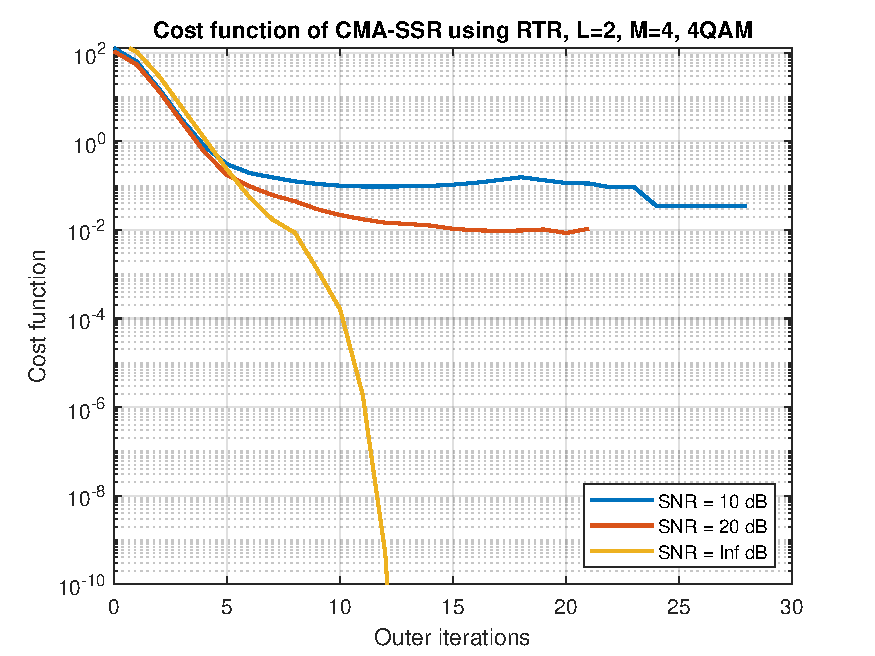
\includegraphics[width=\linewidth]{./figs/BF_RTR_cost_4QAM_L=2_M=4_K=200.pdf}
		\subcaption{Cost function for $K=200$.}
		\label{fig:rtr_cost200}
	\end{subfigure}
	\begin{subfigure}[b]{0.45\textwidth}
		% Caption before figure
		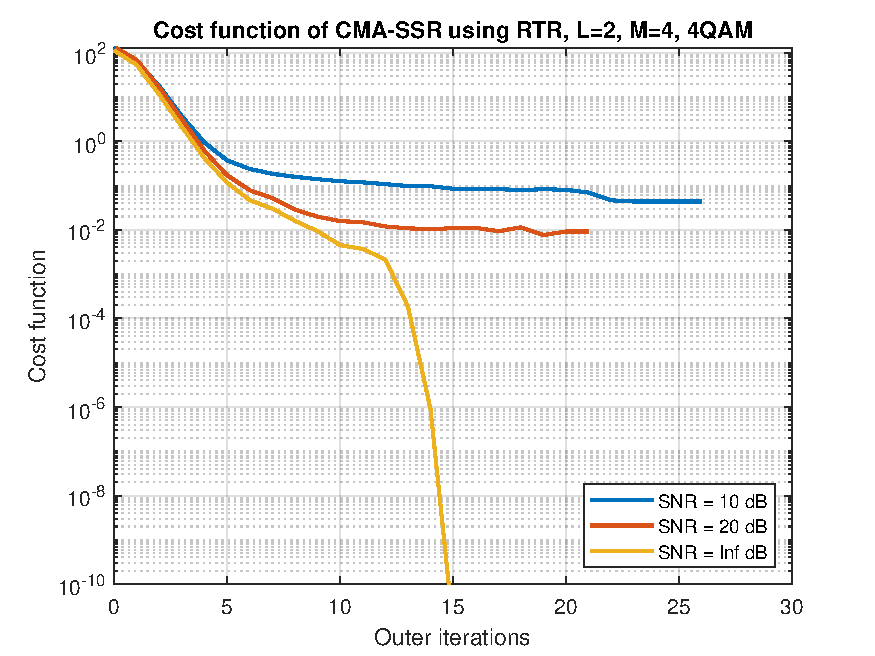
\includegraphics[width=\linewidth]{./figs/BF_RTR_cost_4QAM_L=2_M=4_K=1000.pdf}
		\subcaption{Cost function for $K=1000$.}
		\label{fig:rtr_cost1000}
	\end{subfigure}\\
	\begin{subfigure}[b]{0.45\textwidth}
		% Caption before figure
		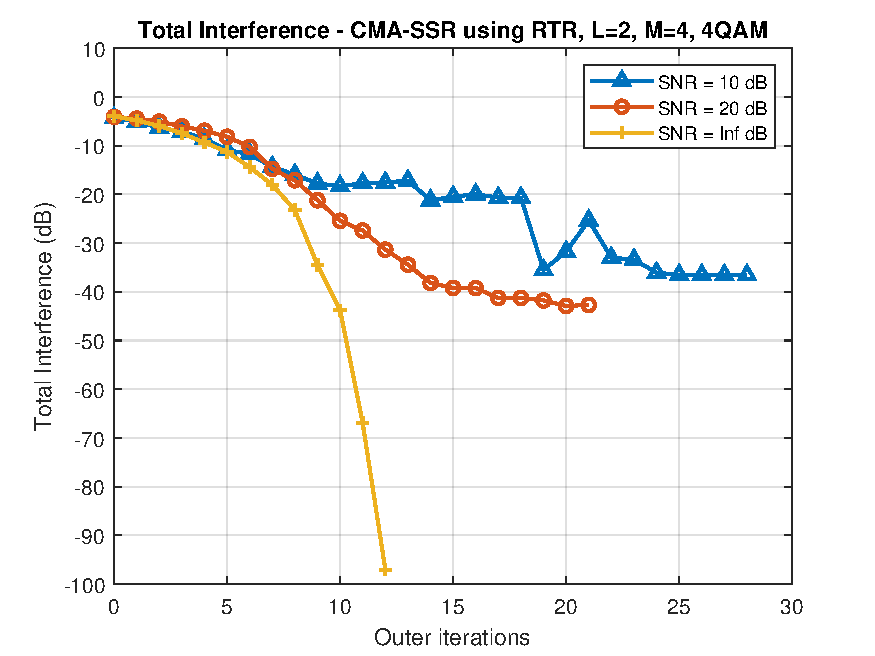
\includegraphics[width=\linewidth]{./figs/BF_RTR_TI_4QAM_L=2_M=4_K=200.pdf}
		\subcaption{Total Interference for $K=200$.}
		\label{fig:rtr_ti200}
	\end{subfigure}
	\begin{subfigure}[b]{0.45\textwidth}
		% Caption before figure
		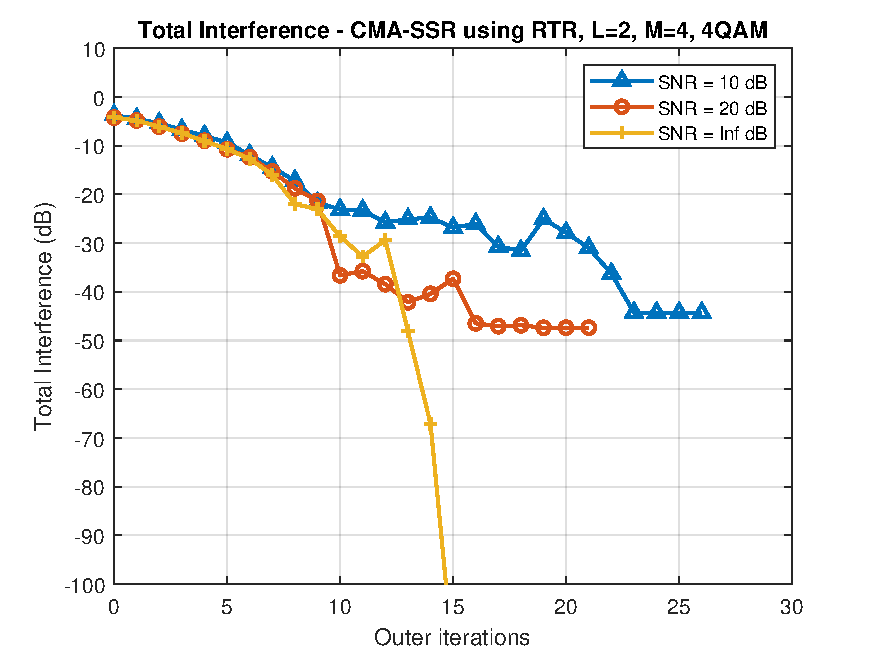
\includegraphics[width=\linewidth]{./figs/BF_RTR_TI_4QAM_L=2_M=4_K=1000.pdf}
		\subcaption{Total Interference for $K=1000$.}
		\label{fig:rtr_ti1000}
	\end{subfigure}
	\begin{subfigure}[b]{0.45\textwidth}
		% Caption before figure
		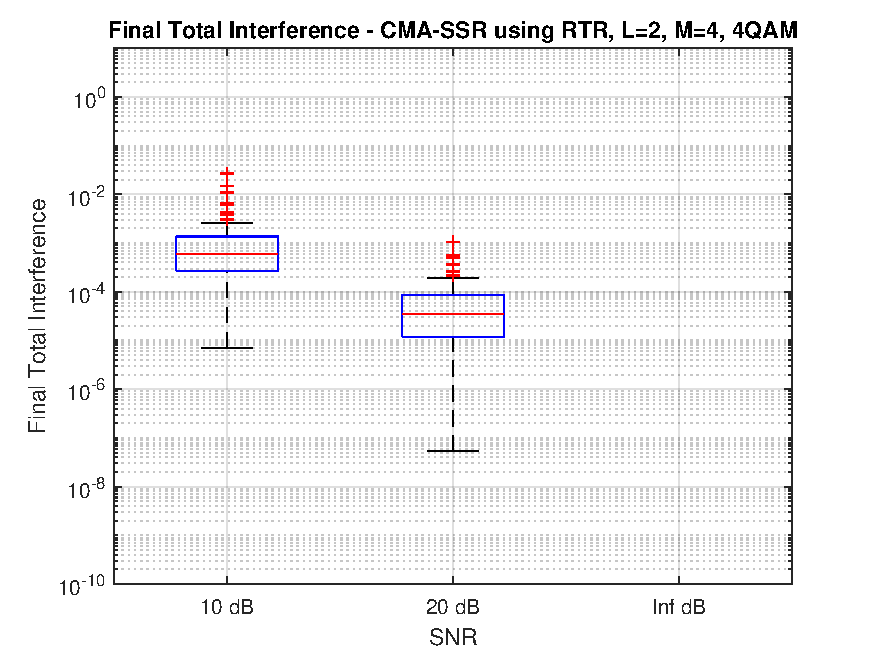
\includegraphics[width=\linewidth]{./figs/BF_RTR_TIfinal_4QAM_L=2_M=4_K=200.pdf}
		\subcaption{Distribution of Interference for $K=200$.}
		\label{fig:rtr_tidist200}
	\end{subfigure}
	\begin{subfigure}[b]{0.45\textwidth}
		% Caption before figure
		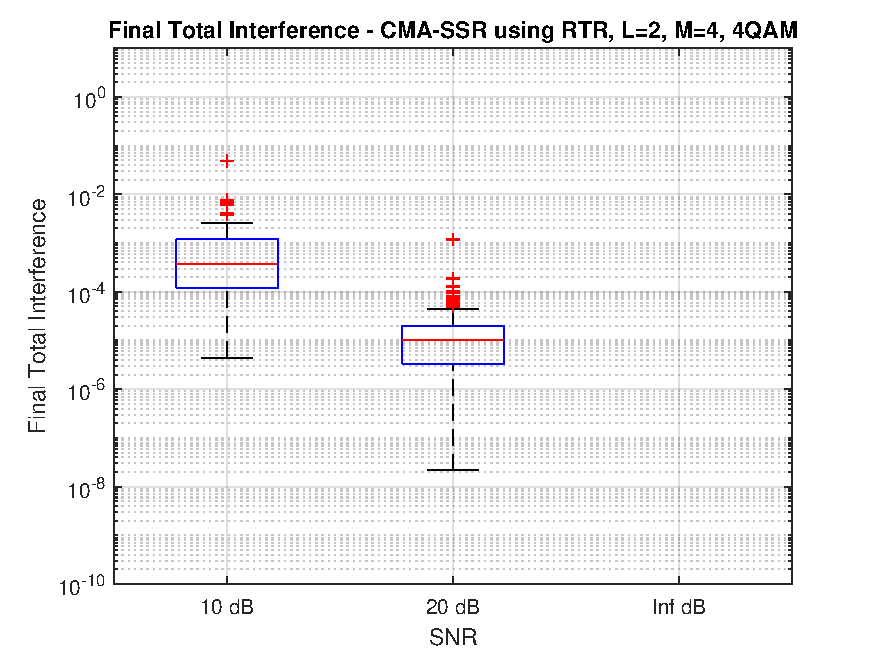
\includegraphics[width=\linewidth]{./figs/BF_RTR_TIfinal_4QAM_L=2_M=4_K=1000.pdf}
		\subcaption{Distribution of interference for $K=1000$.}
		\label{fig:rtr_tidist1000}
	\end{subfigure}
	\caption{Comparison between amount of samples for RTR-SSR convergence. These are mean results from 100 independent runs of the algorithm, with QPSK modulation, $L=2$ and $M=4$.}
	\label{fig:CMA_RTR_qpsk_L2M4}
\end{figure}

\begin{figure}
	\centering
	\begin{subfigure}[b]{0.45\textwidth}
		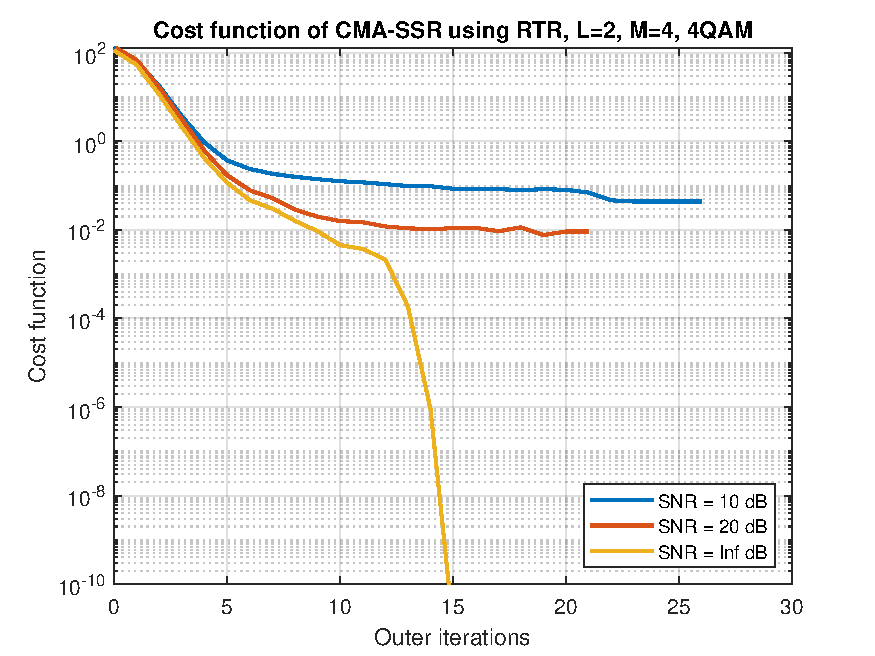
\includegraphics[width=\linewidth]{./figs/BF_RTR_cost_4QAM_L=2_M=4_K=1000.pdf}
		\subcaption{Cost function for QPSK.}
		\label{fig:rtr_costqpsk}
	\end{subfigure}
	\begin{subfigure}[b]{0.45\textwidth}
		% Caption before figure
		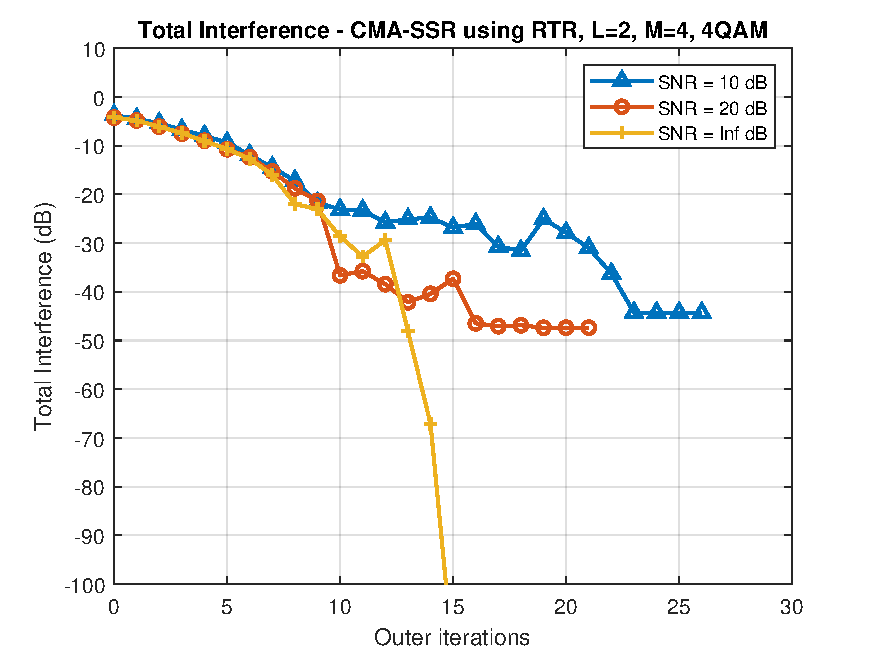
\includegraphics[width=\linewidth]{./figs/BF_RTR_TI_4QAM_L=2_M=4_K=1000.pdf}
		\subcaption{Total interference for QPSK.}
		\label{fig:rtr_ti_qpsk}
	\end{subfigure}\\
	\begin{subfigure}[b]{0.45\textwidth}
		% Caption before figure
		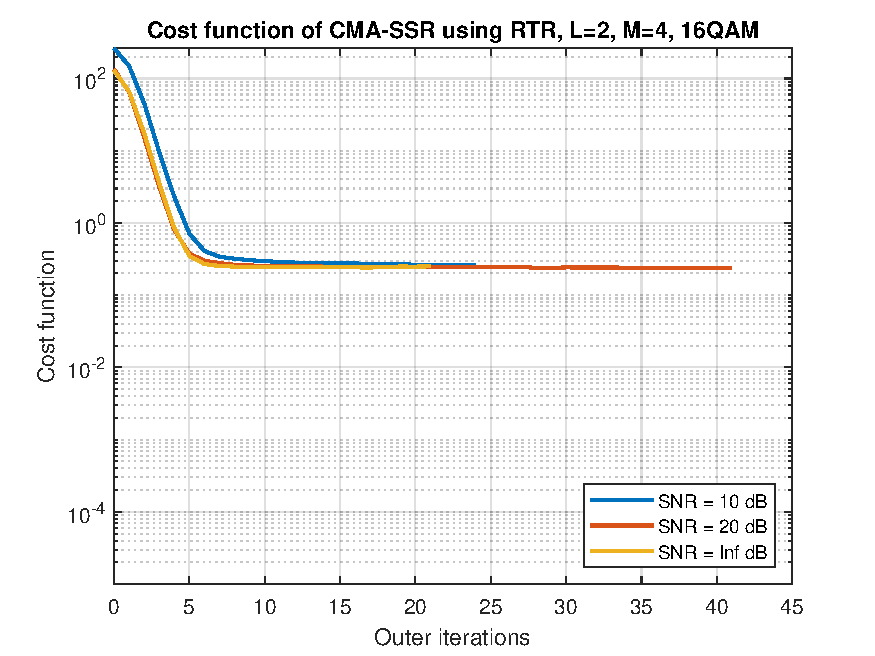
\includegraphics[width=\linewidth]{./figs/BF_RTR_cost_16QAM_L=2_M=4_K=1000.pdf}
		\subcaption{Cost function for 16QAM.}
		\label{fig:rtr_cost16}
	\end{subfigure}
	\begin{subfigure}[b]{0.45\textwidth}
		% Caption before figure
		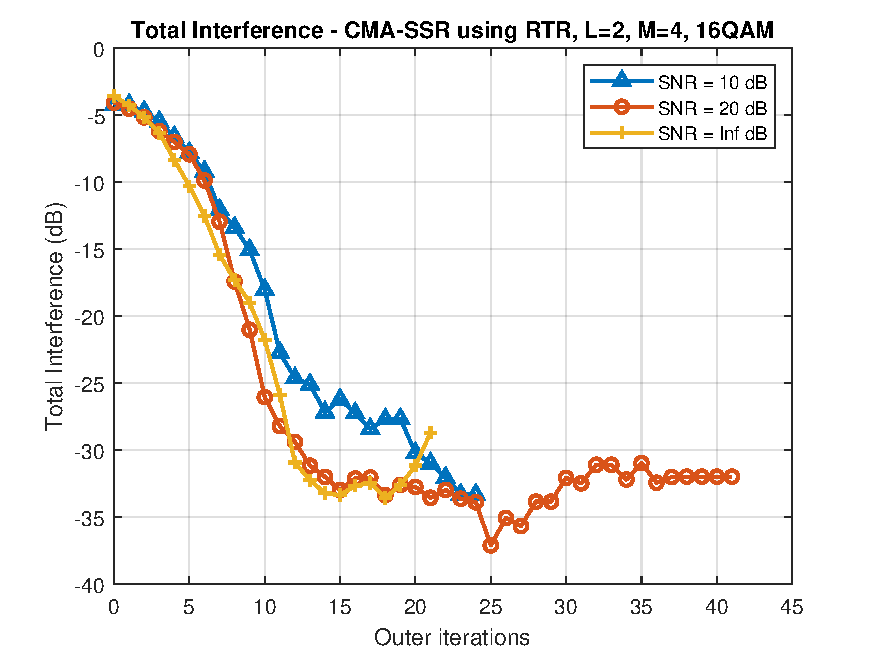
\includegraphics[width=\linewidth]{./figs/BF_RTR_TI_16QAM_L=2_M=4_K=1000.pdf}
		\subcaption{Total interference for 16QAM.}
		\label{fig:rtr_ti16}
	\end{subfigure}
	\begin{subfigure}[b]{0.45\textwidth}
		% Caption before figure
		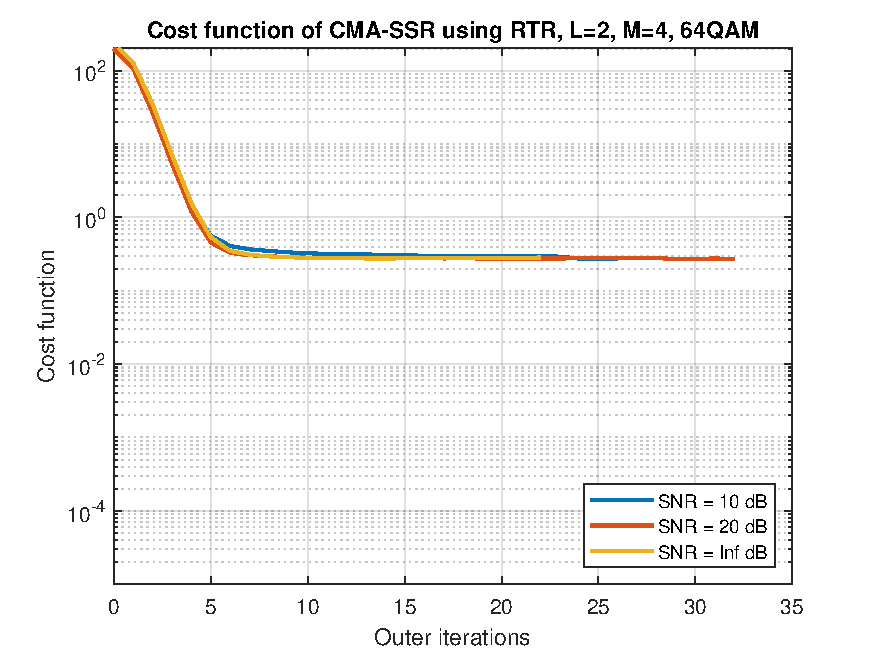
\includegraphics[width=\linewidth]{./figs/BF_RTR_cost_64QAM_L=2_M=4_K=1000.pdf}
		\subcaption{Cost function for 64QAM.}
		\label{fig:rtr_cost64}
	\end{subfigure}
	\begin{subfigure}[b]{0.45\textwidth}
		% Caption before figure
		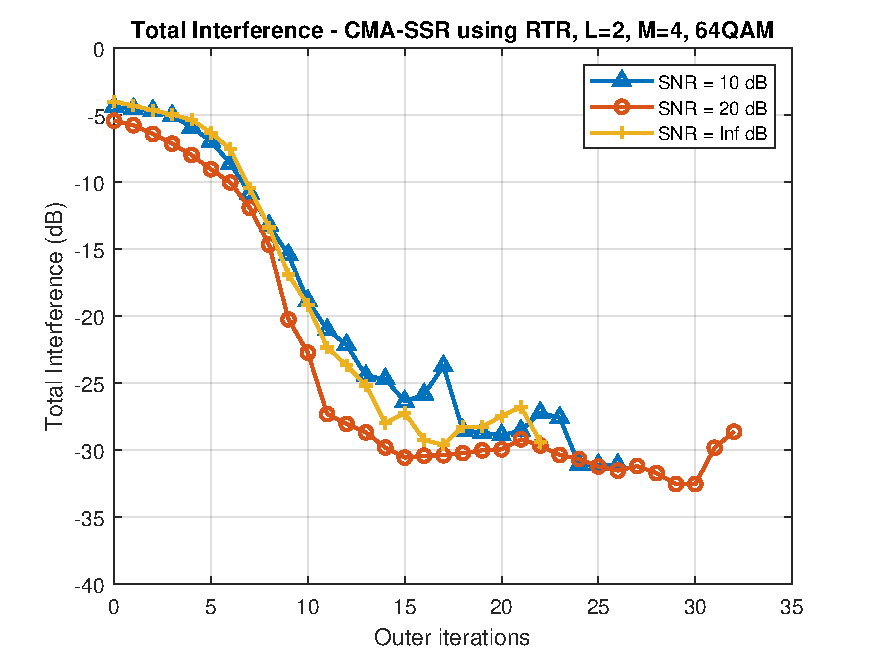
\includegraphics[width=\linewidth]{./figs/BF_RTR_TI_64QAM_L=2_M=4_K=1000.pdf}
		\subcaption{Total interference for 64QAM.}
		\label{fig:rtr_ti64}
	\end{subfigure}
	\caption{Comparison between modulations for RTR-SSR convergence. These are mean results from 100 independent runs of the algorithm, with different SNR values, $K=1000$, $L=2$ and $M=4$.}
	\label{fig:CMA_RTR_mods_L2M4}
\end{figure}

\begin{figure}
	\centering
	\begin{subfigure}[b]{0.45\textwidth}
		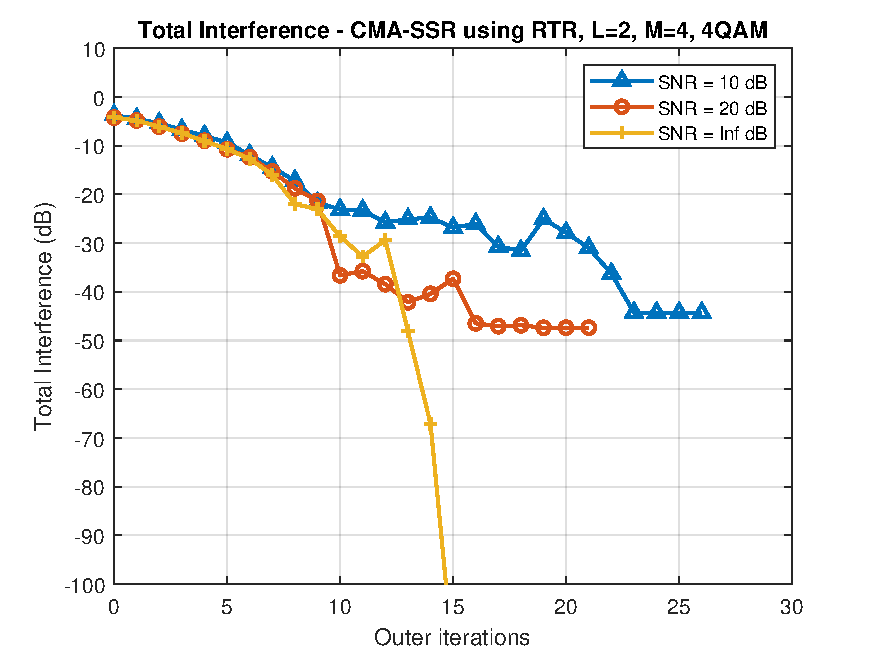
\includegraphics[width=\linewidth]{./figs/BF_RTR_TI_4QAM_L=2_M=4_K=1000.pdf}
	\subcaption{TI, QPSK, $L=2$, $M=4$.}
		\label{fig:rtr_ti4_24}
	\end{subfigure}
	\begin{subfigure}[b]{0.45\textwidth}
		% Caption before figure
		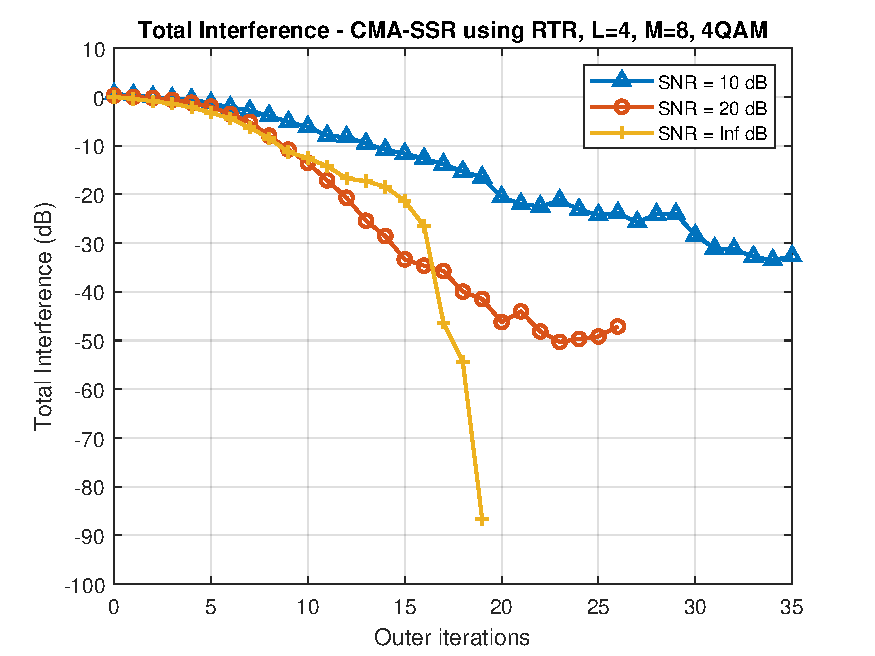
\includegraphics[width=\linewidth]{./figs/BF_RTR_TI_4QAM_L=4_M=8_K=1000.pdf}
	\subcaption{TI, QPSK, $L=4$, $M=8$.}
		\label{fig:rtr_ti4_48}
	\end{subfigure}\\
	\begin{subfigure}[b]{0.45\textwidth}
		% Caption before figure
		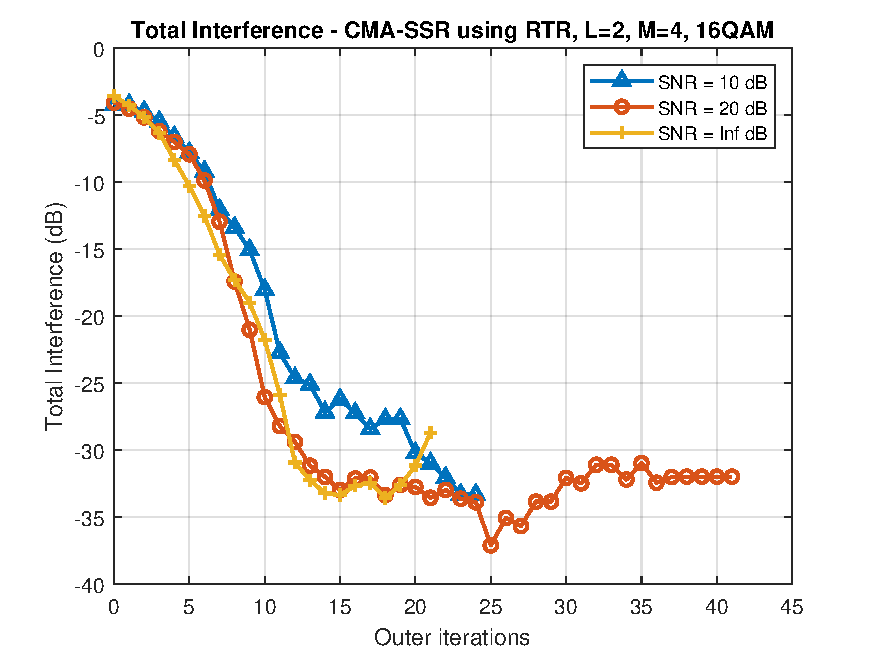
\includegraphics[width=\linewidth]{./figs/BF_RTR_TI_16QAM_L=2_M=4_K=1000.pdf}
	\subcaption{TI, 16QAM, $L=2$, $M=4$.}
		\label{fig:rtr_ti16_24}
	\end{subfigure}
	\begin{subfigure}[b]{0.45\textwidth}
		% Caption before figure
		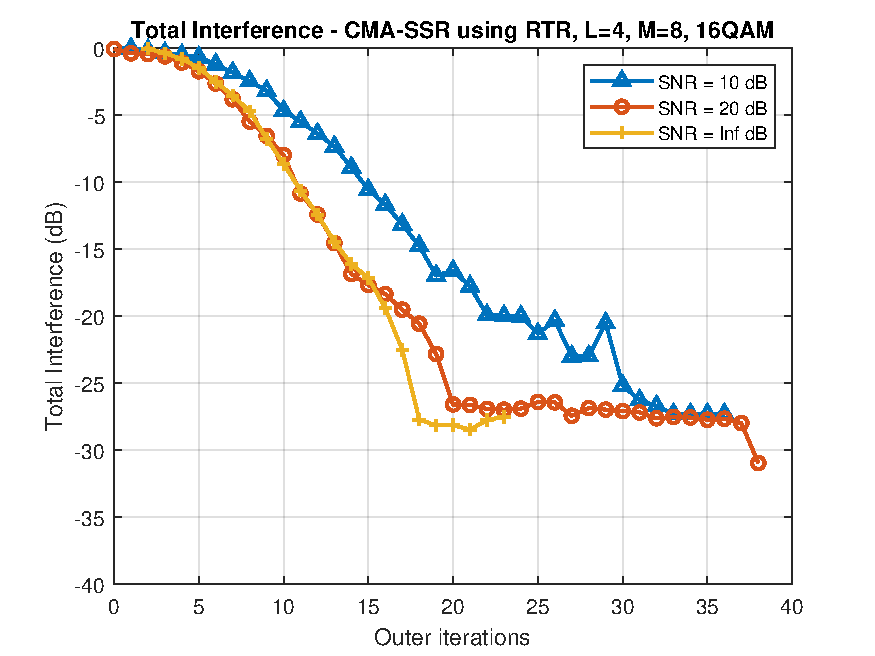
\includegraphics[width=\linewidth]{./figs/BF_RTR_TI_16QAM_L=4_M=8_K=1000.pdf}
	\subcaption{TI, 16QAM, $L=42$, $M=8$.}
		\label{fig:rtr_ti16_48}
	\end{subfigure}
	\begin{subfigure}[b]{0.45\textwidth}
		% Caption before figure
		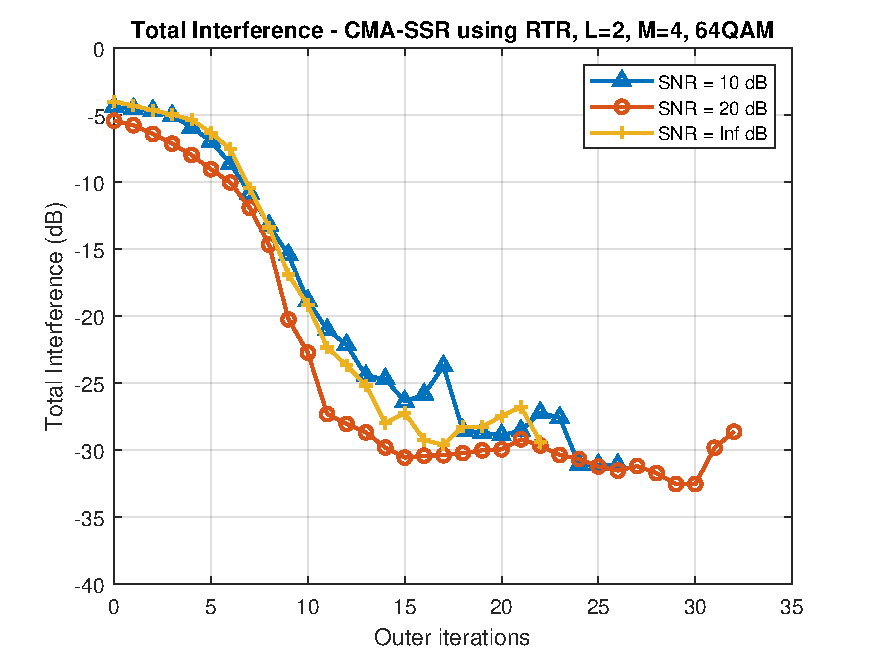
\includegraphics[width=\linewidth]{./figs/BF_RTR_TI_64QAM_L=2_M=4_K=1000.pdf}
	\subcaption{TI, 64QAM, $L=2$, $M=4$.}
		\label{fig:rtr_ti64_24}
	\end{subfigure}
	\begin{subfigure}[b]{0.45\textwidth}
		% Caption before figure
		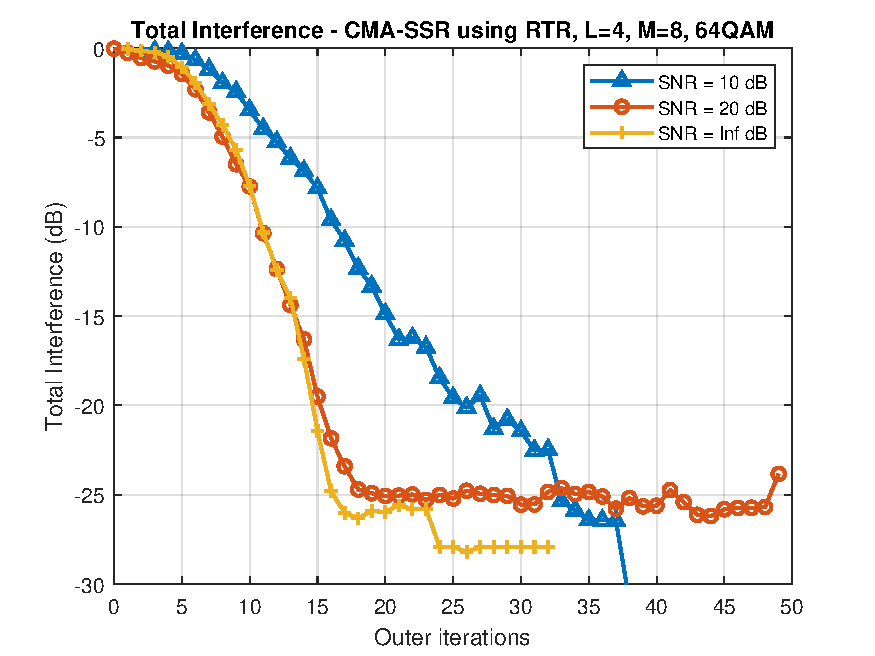
\includegraphics[width=\linewidth]{./figs/BF_RTR_TI_64QAM_L=4_M=8_K=1000.pdf}
		\subcaption{TI, 64QAM, $L=4$, $M=8$.}
		\label{fig:rtr_ti64_48}
	\end{subfigure}
	\caption{Comparison between system sizes for RTR-SSR convergence. These are mean results from 100 independent runs of the algorithm, with different SNR values and $K=1000$.}
	\label{fig:CMA_RTR_size_qpsk}
\end{figure}

\newpage
\subsection{Multiple source recovery}\label{sim:RTR_MSR}
Here, we replicate some results from the single source recovery experiments, but recovering multiple sources at a time. We furthermore set $\gamma_0=1$.

Figure~\ref{fig:CMA_RTR_msr_qpsk_L2M4} presents the cost function value and the total interference vs. outer iterations for each SNR value in a random experiment with QPSK transmissions, $L=2$ sources and $M=4$ receiving antennas. The left column shows the experiment using $K=200$ samples and the right column shows the experiment using $K=1000$ samples. This shows that the RTR algorithm converges for all SNR values in as few as 30 outer iterations or less in average, even with a lower number of available samples. The total interference decays rapidly over iterations, and the final interference obtained (when RTR meets the stopping criterion) is less than 30dB with high probability around all cases.

Figure~\ref{fig:CMA_RTR_msr_mods_L2M4} shows the behavior of WF for different modulation schemes, with $K=1000$, $L=2$ and $M=4$. Over all modulations, it takes less than 40 outer iterations to satisfiy the stopping criterion, and it takes 30 iterations or less to achieve -25dB of total interference in average.

Finally, Figure~\ref{fig:CMA_RTR_msr_size_qpsk} shows the effect of the system size $M\times L$ on the behavior of RTR. As mentioned above, a greater number of sources implies more interference to get rid of, effect we see again in both equalizers across across modulation schemes and SNR values. Nevertheless, these results show the capability of RTR when applied to CMA-based multiple source recovery.

\begin{figure}
	\centering
	\begin{subfigure}[b]{0.45\textwidth}
		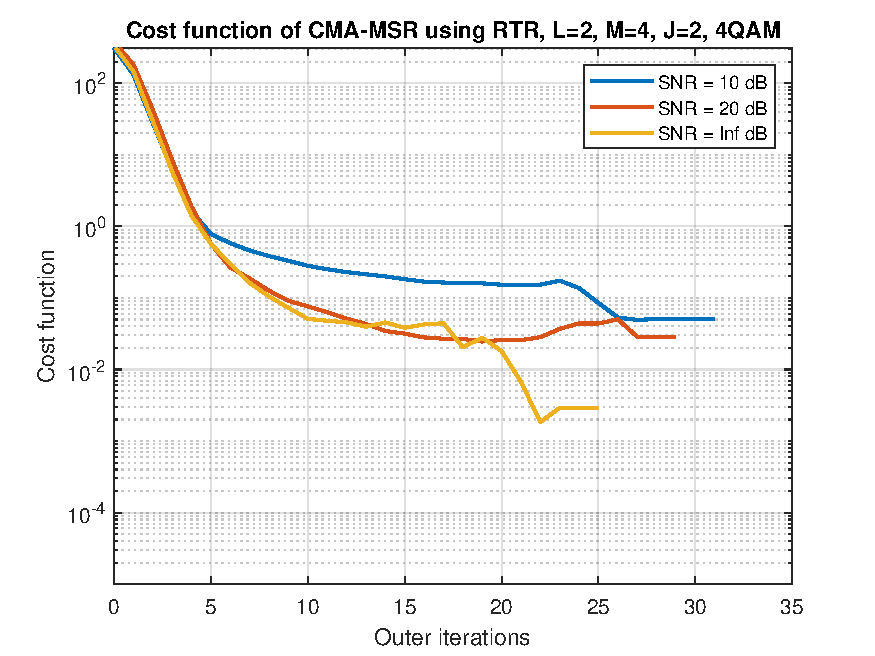
\includegraphics[width=\linewidth]{./figs/BF_RTR_MSR_cost_4QAM_L=2_M=4_J=2_K=200.pdf}
		\subcaption{Cost function for $K=200$.}
		\label{fig:rtr_msr_cost200}
	\end{subfigure}
	\begin{subfigure}[b]{0.45\textwidth}
		% Caption before figure
		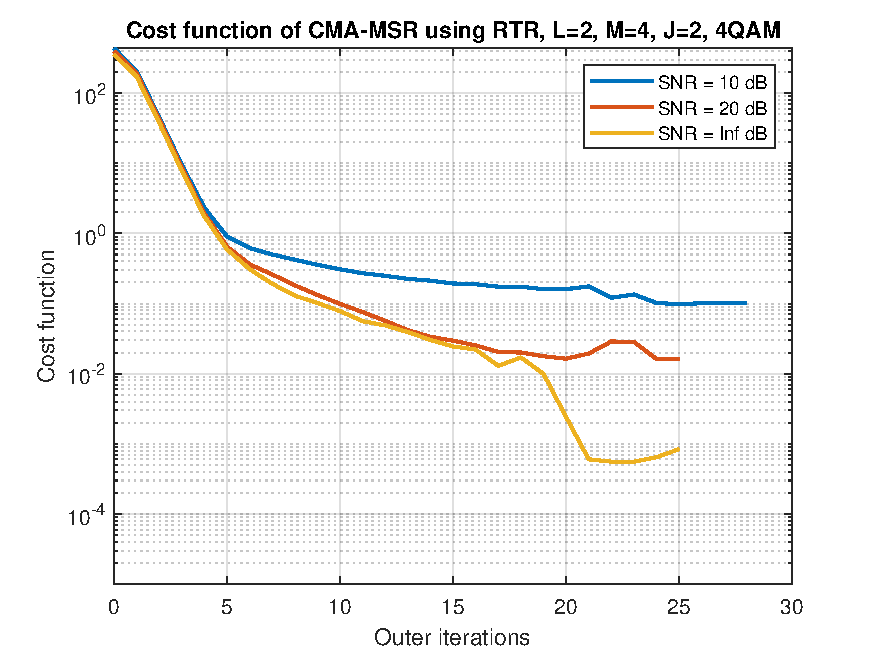
\includegraphics[width=\linewidth]{./figs/BF_RTR_MSR_cost_4QAM_L=2_M=4_J=2_K=1000.pdf}
		\subcaption{Cost function for $K=1000$.}
		\label{fig:rtr_msr_cost1000}
	\end{subfigure}\\
	\begin{subfigure}[b]{0.45\textwidth}
		% Caption before figure
		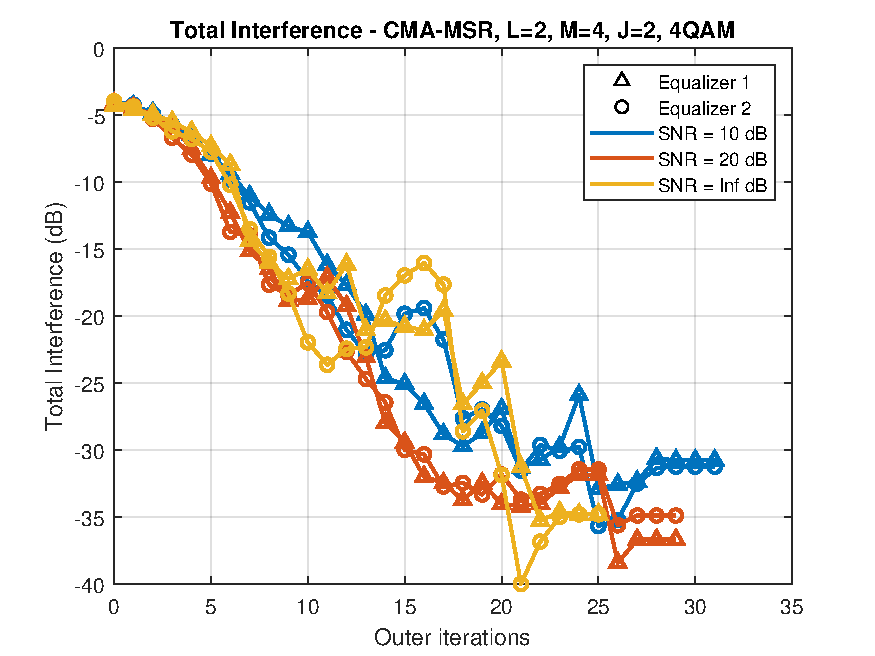
\includegraphics[width=\linewidth]{./figs/BF_RTR_MSR_TI_4QAM_L=2_M=4_J=2_K=200.pdf}
		\subcaption{Total Interference for $K=200$.}
		\label{fig:rtr_msr_ti200}
	\end{subfigure}
	\begin{subfigure}[b]{0.45\textwidth}
		% Caption before figure
		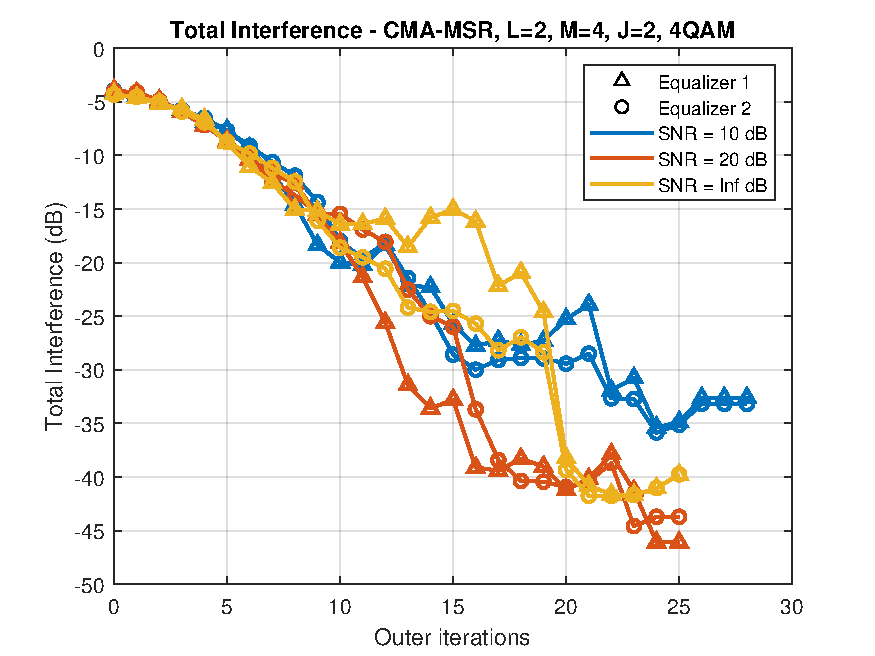
\includegraphics[width=\linewidth]{./figs/BF_RTR_MSR_TI_4QAM_L=2_M=4_J=2_K=1000.pdf}
		\subcaption{Total Interference for $K=1000$.}
		\label{fig:rtr_msr_ti1000}
	\end{subfigure}
	\begin{subfigure}[b]{0.45\textwidth}
		% Caption before figure
		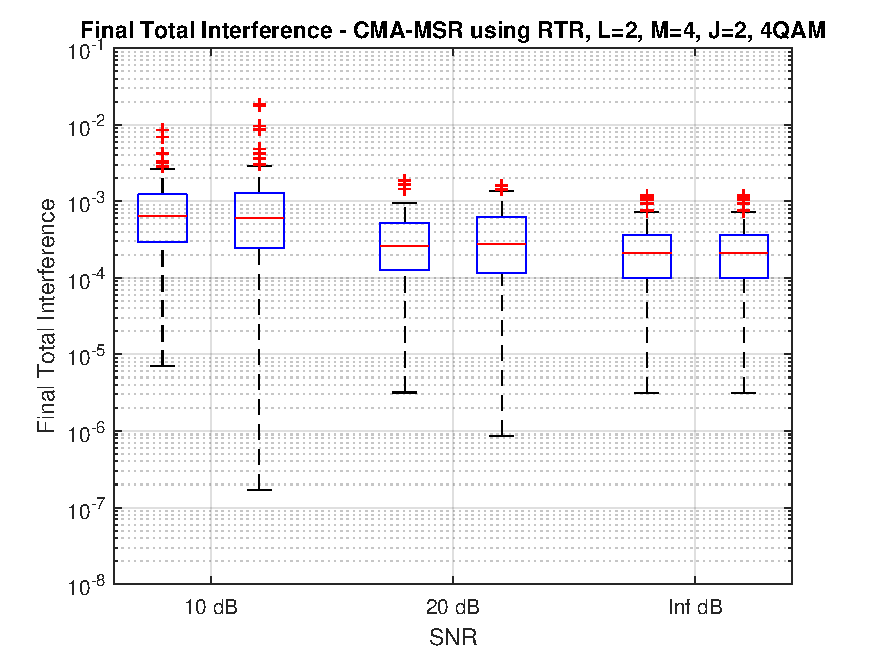
\includegraphics[width=\linewidth]{./figs/BF_RTR_MSR_TIfinal_4QAM_L=2_M=4_J=2_K=200.pdf}
		\subcaption{Distribution of Interference for $K=200$.}
		\label{fig:rtr_msr_tidist200}
	\end{subfigure}
	\begin{subfigure}[b]{0.45\textwidth}
		% Caption before figure
		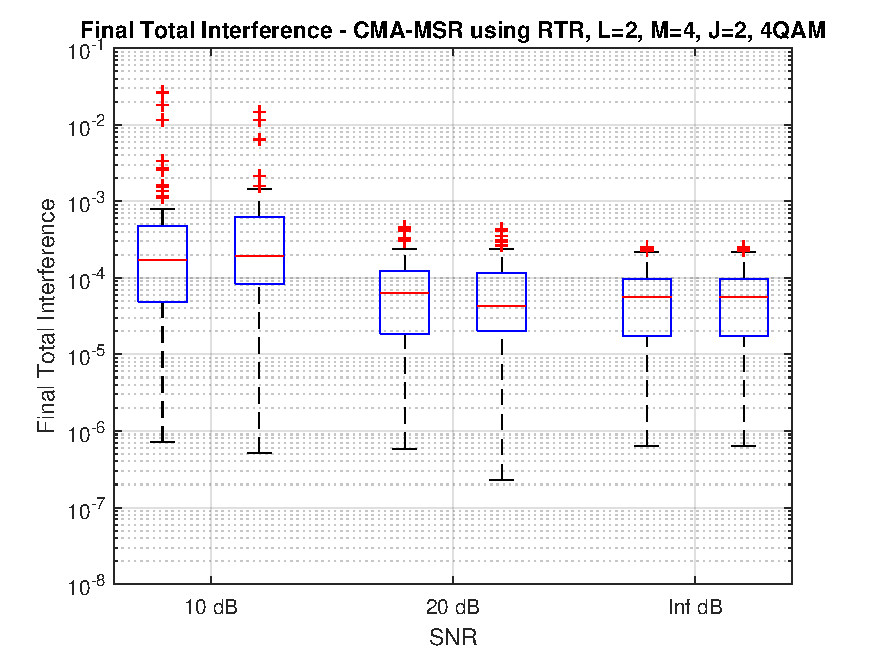
\includegraphics[width=\linewidth]{./figs/BF_RTR_MSR_TIfinal_4QAM_L=2_M=4_J=2_K=1000.pdf}
		\subcaption{Distribution of interference for $K=1000$.}
		\label{fig:rtr_msr_tidist1000}
	\end{subfigure}
	\caption{Comparison between amount of samples for RTR-MSR convergence. These are mean results from 100 independent runs of the algorithm, with QPSK modulation, $L=2$, $J=2$ and $M=4$.}
	\label{fig:CMA_RTR_msr_qpsk_L2M4}
\end{figure}

\begin{figure}
	\centering
	\begin{subfigure}[b]{0.45\textwidth}
		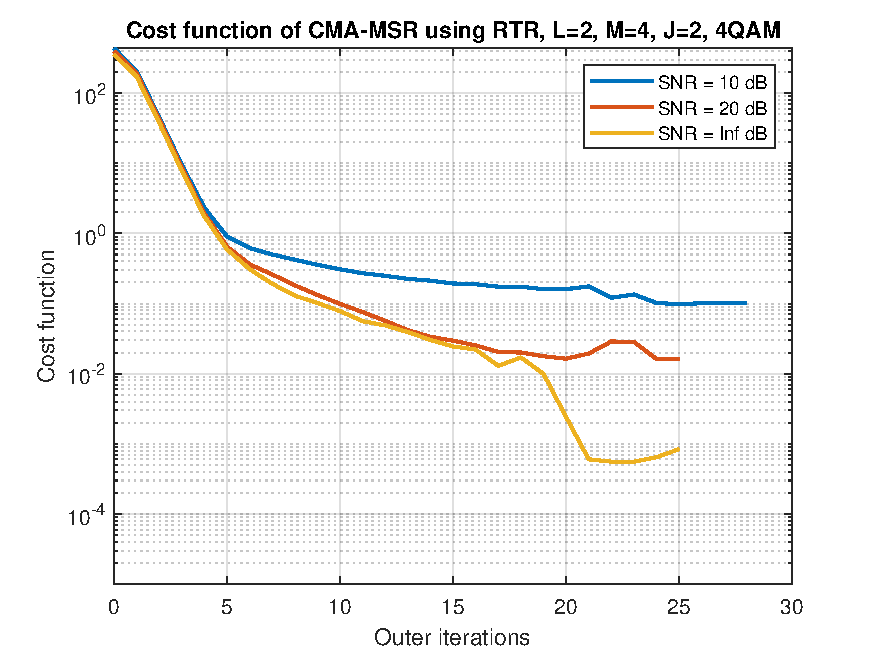
\includegraphics[width=\linewidth]{./figs/BF_RTR_MSR_cost_4QAM_L=2_M=4_J=2_K=1000.pdf}
		\subcaption{Cost function for QPSK.}
		\label{fig:rtr_msr_costqpsk}
	\end{subfigure}
	\begin{subfigure}[b]{0.45\textwidth}
		% Caption before figure
		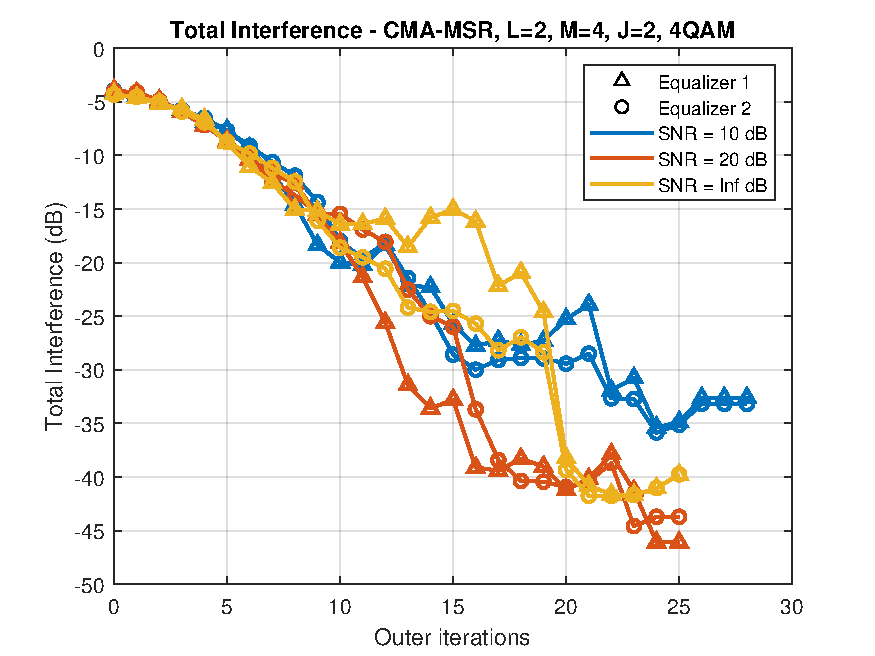
\includegraphics[width=\linewidth]{./figs/BF_RTR_MSR_TI_4QAM_L=2_M=4_J=2_K=1000.pdf}
		\subcaption{Total interference for QPSK.}
		\label{fig:rtr_msr_ti_qpsk}
	\end{subfigure}\\
	\begin{subfigure}[b]{0.45\textwidth}
		% Caption before figure
		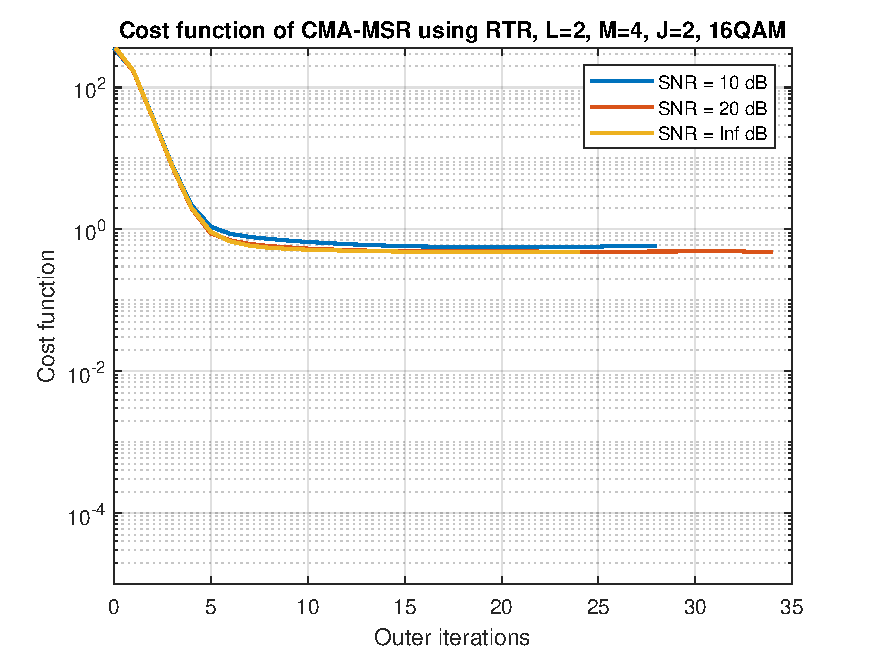
\includegraphics[width=\linewidth]{./figs/BF_RTR_MSR_cost_16QAM_L=2_M=4_J=2_K=1000.pdf}
		\subcaption{Cost function for 16QAM.}
		\label{fig:rtr_msr_cost16}
	\end{subfigure}
	\begin{subfigure}[b]{0.45\textwidth}
		% Caption before figure
		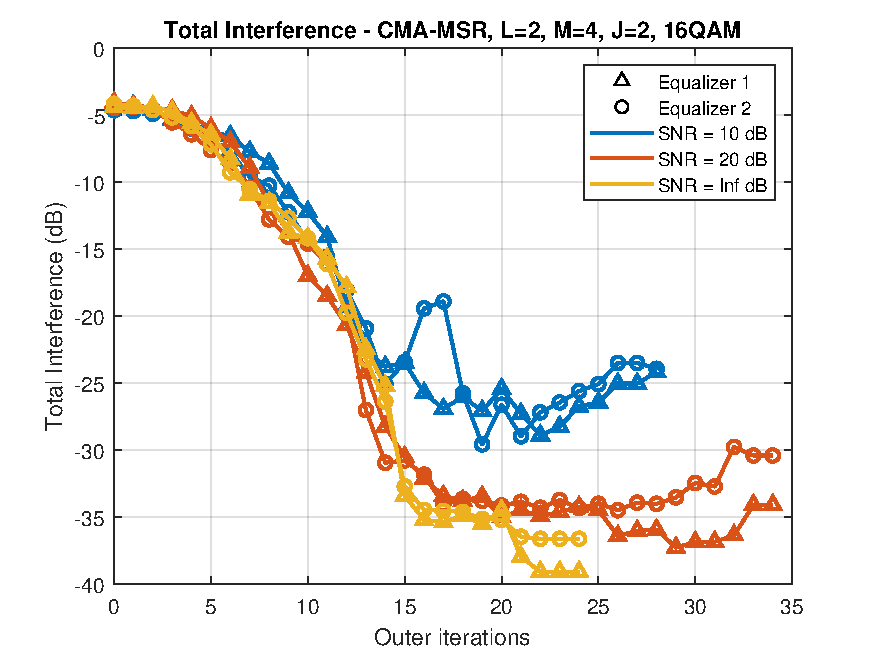
\includegraphics[width=\linewidth]{./figs/BF_RTR_MSR_TI_16QAM_L=2_M=4_J=2_K=1000.pdf}
		\subcaption{Total interference for 16QAM.}
		\label{fig:rtr_msr_ti16}
	\end{subfigure}
	\begin{subfigure}[b]{0.45\textwidth}
		% Caption before figure
		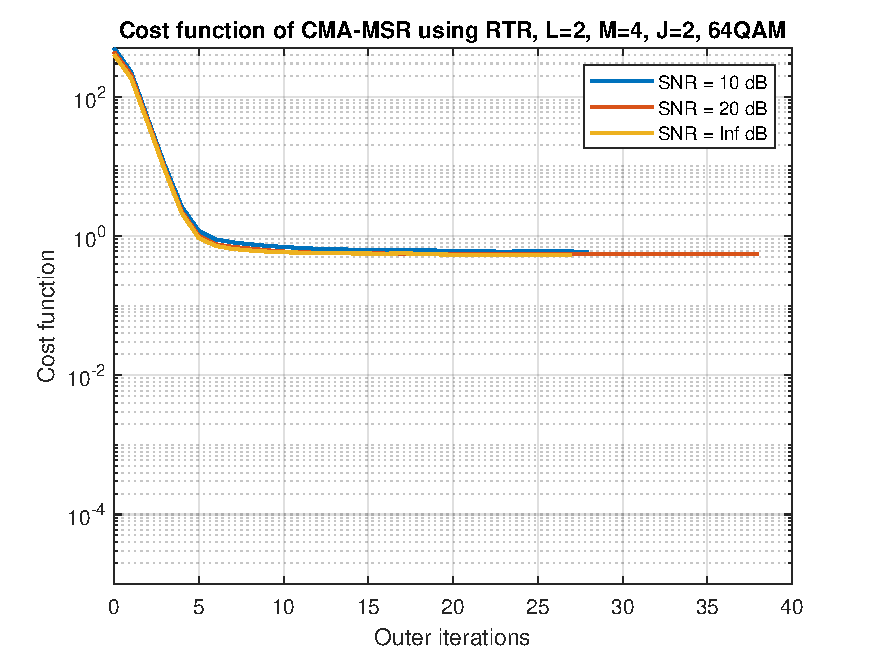
\includegraphics[width=\linewidth]{./figs/BF_RTR_MSR_cost_64QAM_L=2_M=4_J=2_K=1000.pdf}
		\subcaption{Cost function for 64QAM.}
		\label{fig:rtr_msr_cost64}
	\end{subfigure}
	\begin{subfigure}[b]{0.45\textwidth}
		% Caption before figure
		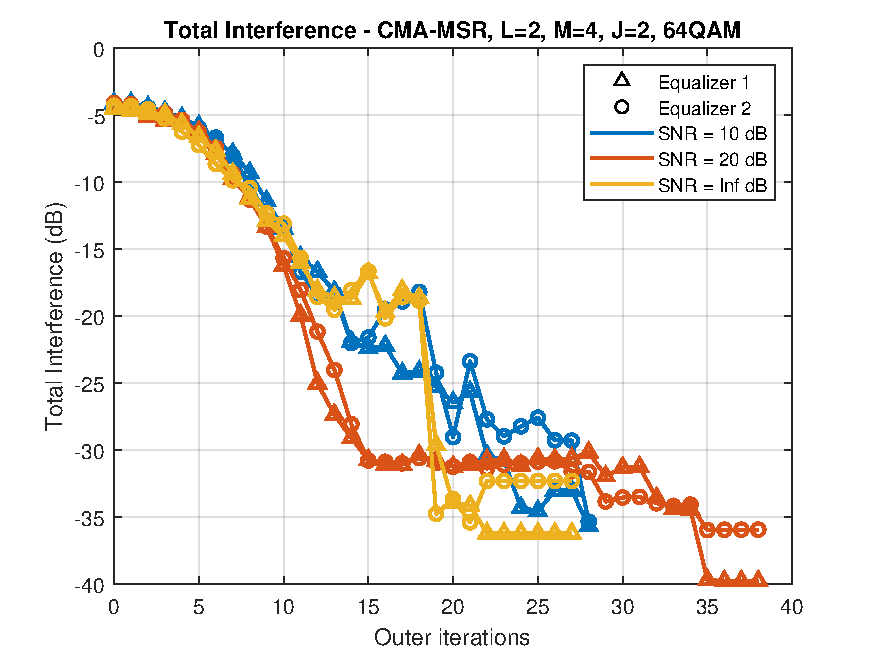
\includegraphics[width=\linewidth]{./figs/BF_RTR_MSR_TI_64QAM_L=2_M=4_J=2_K=1000.pdf}
		\subcaption{Total interference for 64QAM.}
		\label{fig:rtr_msr_ti64}
	\end{subfigure}
	\caption{Comparison between modulations for RTR-MSR convergence. These are mean results from 100 independent runs of the algorithm, with different SNR values, $K=1000$, $L=2$, $J=2$ and $M=4$.}
	\label{fig:CMA_RTR_msr_mods_L2M4}
\end{figure}

\begin{figure}
	\centering
	\begin{subfigure}[b]{0.45\textwidth}
		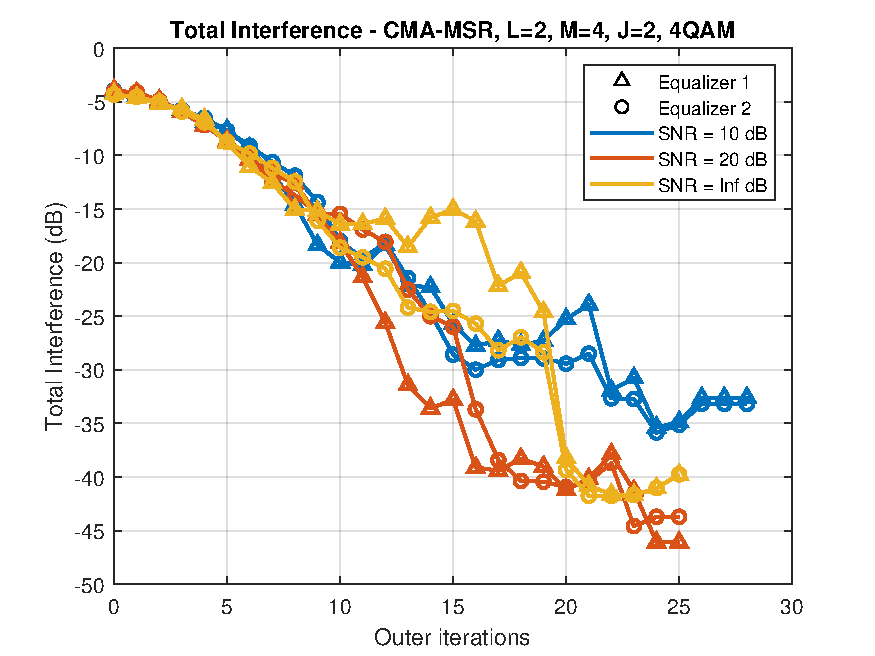
\includegraphics[width=\linewidth]{./figs/BF_RTR_MSR_TI_4QAM_L=2_M=4_J=2_K=1000.pdf}
		\subcaption{TI, QPSK, $L=2$, $M=4$.}
		\label{fig:rtr_msr_ti4_24}
	\end{subfigure}
	\begin{subfigure}[b]{0.45\textwidth}
		% Caption before figure
		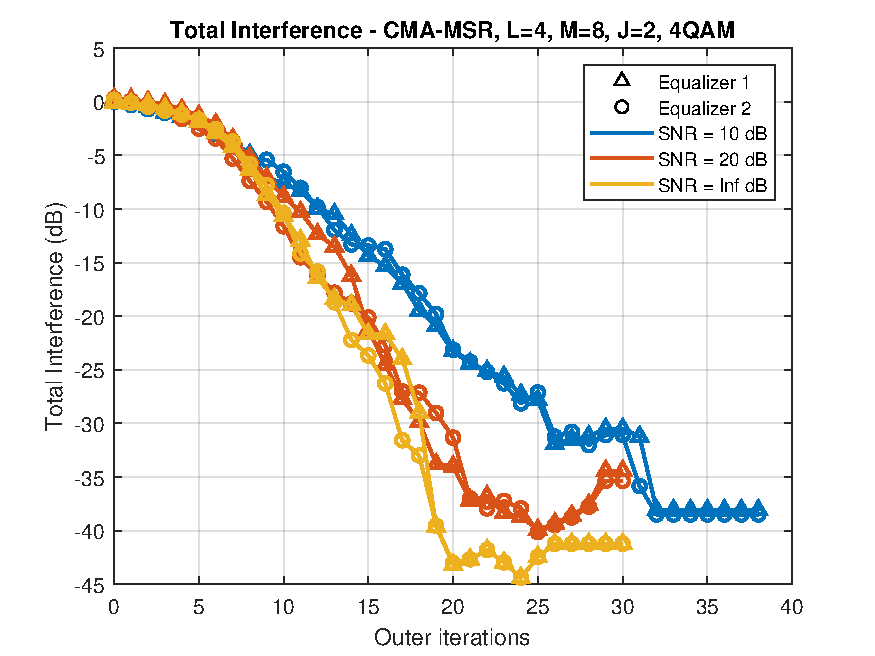
\includegraphics[width=\linewidth]{./figs/BF_RTR_MSR_TI_4QAM_L=4_M=8_J=2_K=1000.pdf}
		\subcaption{TI, QPSK, $L=4$, $M=8$.}
		\label{fig:rtr_msr_ti4_48}
	\end{subfigure}\\
	\begin{subfigure}[b]{0.45\textwidth}
		% Caption before figure
		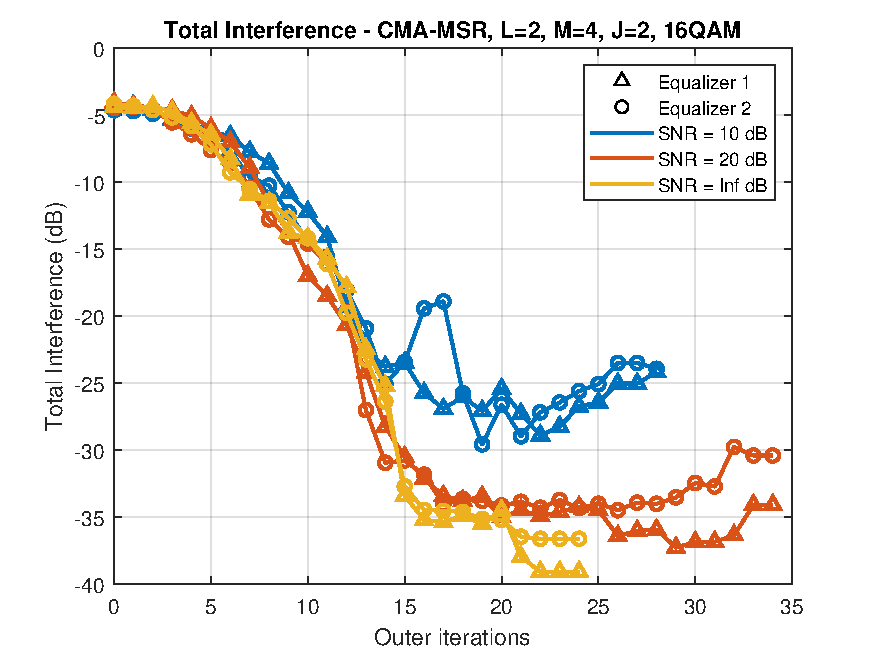
\includegraphics[width=\linewidth]{./figs/BF_RTR_MSR_TI_16QAM_L=2_M=4_J=2_K=1000.pdf}
		\subcaption{TI, 16QAM, $L=2$, $M=4$.}
		\label{fig:rtr_msr_ti16_24}
	\end{subfigure}
	\begin{subfigure}[b]{0.45\textwidth}
		% Caption before figure
		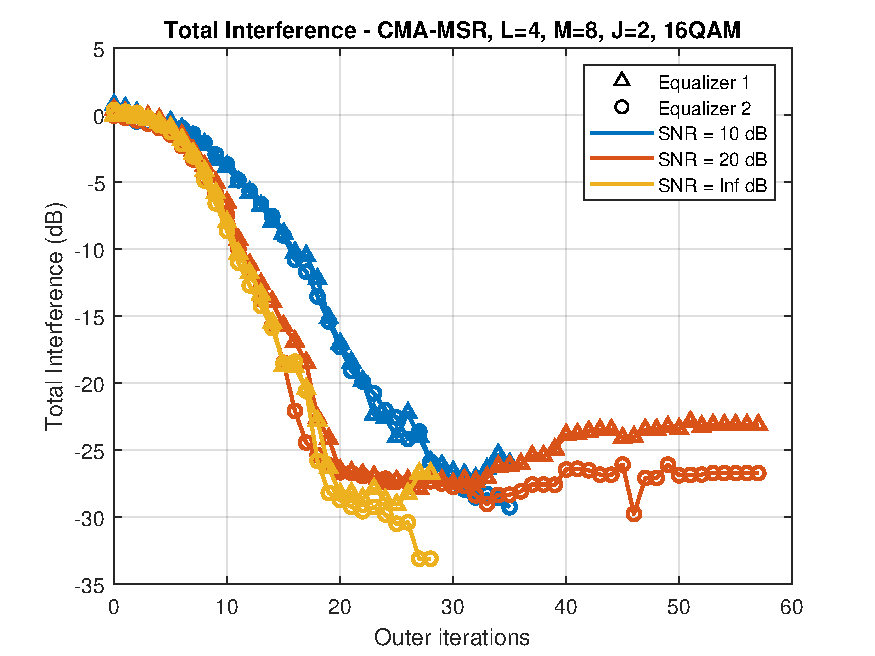
\includegraphics[width=\linewidth]{./figs/BF_RTR_MSR_TI_16QAM_L=4_M=8_J=2_K=1000.pdf}
		\subcaption{TI, 16QAM, $L=4$, $M=8$.}
		\label{fig:rtr_msr_ti16_48}
	\end{subfigure}
	\begin{subfigure}[b]{0.45\textwidth}
		% Caption before figure
		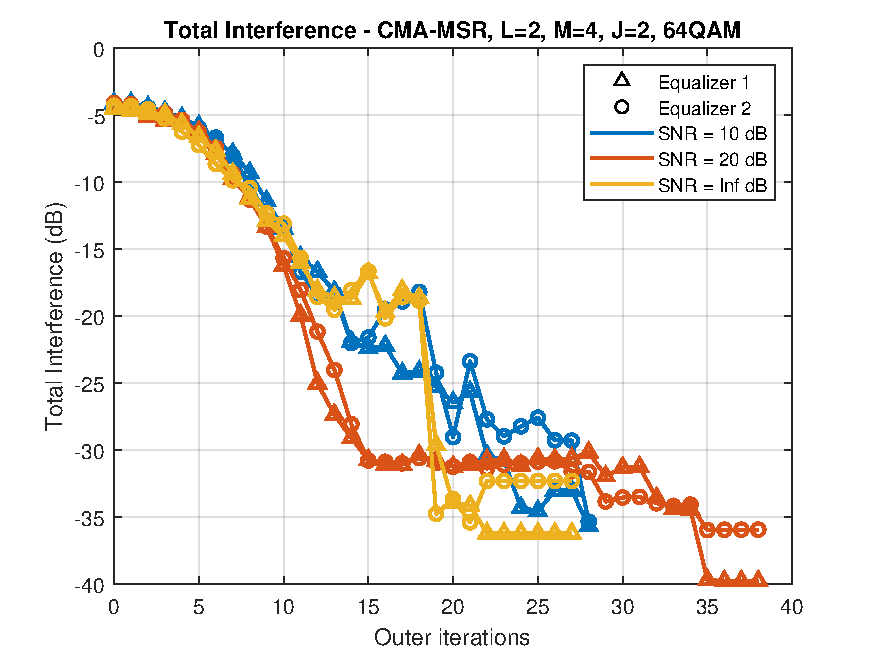
\includegraphics[width=\linewidth]{./figs/BF_RTR_MSR_TI_64QAM_L=2_M=4_J=2_K=1000.pdf}
		\subcaption{TI, 64QAM, $L=2$, $M=4$.}
		\label{fig:rtr_msr_ti64_24}
	\end{subfigure}
	\begin{subfigure}[b]{0.45\textwidth}
		% Caption before figure
		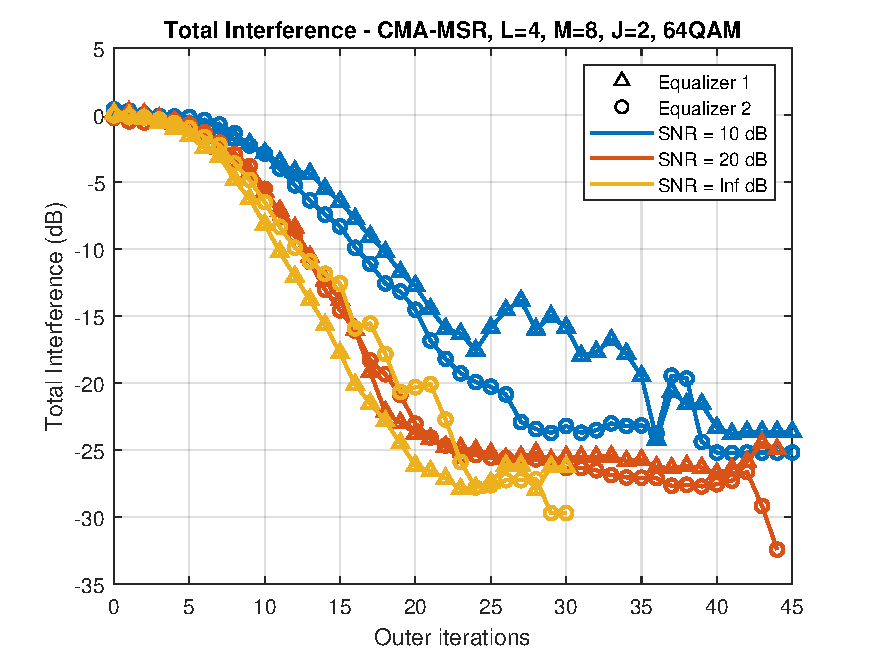
\includegraphics[width=\linewidth]{./figs/BF_RTR_MSR_TI_64QAM_L=4_M=8_J=2_K=1000.pdf}
		\subcaption{TI, 64QAM, $L=4$, $M=8$.}
		\label{fig:rtr_msr_ti64_48}
	\end{subfigure}
	\caption{Comparison between system sizes for RTR-MSR convergence. These are mean results from 100 independent runs of the algorithm, with different SNR values, $J=2$ and $K=1000$.}
	\label{fig:CMA_RTR_msr_size_qpsk}
\end{figure}
